 \documentclass[letterpaper,10pt]{article}

\usepackage{amsmath}
\usepackage[utf8x]{inputenc}
\usepackage{caption}
\usepackage{subcaption}
\usepackage{graphicx}
\usepackage{subfig}
\usepackage{float}
\usepackage{natbib}
\usepackage{anysize}
\usepackage{float}
\usepackage{tabularx}
\usepackage{amsmath}
\usepackage{amssymb}
\usepackage{amsfonts}
\usepackage{mathrsfs}
\usepackage{setspace}
\usepackage{relsize}

\usepackage{multicol}

%
%\marginsize{1.in}{1.in}{1in}{1in}
%\linespread{1.25}
%\setlength\parindent{0pt}


\title{Comparison Between Heuristic and Eulerian Interface Capturing Approaches for Shallow Water Type Flow}
\author{Hossein Aghakhani, Keith Dalbey, Abani Patra, David Salac}
\date{}

\begin{document}

\maketitle

\begin {abstract}{
Determining the wet-dry boundary has historically been a challenge when 
solving the depth-averaged shallow-water (SW) equations (or similar granular flows), and has 
been the focus of much research efforts. In this paper, to the best knowledge of authors, for the first time we used level set and phase field methods to solve this issue and other related problems. We also proposed a new heuristic method to address this problem. We implemented all of these methods in TITAN2D which is a parallel adaptive mesh refinement toolkit designed for numerical simulation of granullar flows.\newline
The results of the methods were presented for simple inclined plane and Colima volcano. For the inclined plane we verified the results with experimental data and for Colima volcano they have been compare with field data. We successfully captured the interface of the flow and solved the accuracy and stability problems related t thin layer problem in SW numerical solution. The comparison of results shows that although all of the methods can be used to address this problems, but each of them has its own advantage/disadvantages that has to be chosen carefully depend to the criteria of the interested case.\newline
\textbf{Keywords:} Shallow water flow, Thin layer, Wetting/Drying, Phase field, Level set}
\end{abstract}

% =============================================================================
%                 INTRODUCTION
% =============================================================================
\section{Introduction} 
\label{introduction}
% Basic introduction about the Shallow water
Shallow water (SW) flows include a wide range of fluid flows. In SW flows the fluid depth is much 
smaller than the characteristic length of the fluid body. In deriving the corresponding 
governing equations, the shallowness of flow allows us to neglect the variation of state variables  in perpendicular direction to the basal surface, and the effect of 
this replaced with an integrated average in the equations \cite{SavageHutter1989}. 
This mathematical simplification allows us to simplify three dimension flow in two dimension.
The aforementioned condition holds for many circumstances in geophysical flow and the same 
conservation equations with some minor modifications could be used to study this type of flow. \newline
To this aim, Eglit and Sveshnikova \cite{eglit1980mms} modified the depth-averaged Saint Venant equations to simulate granular snow avalanches, and almost a decade later Savage and Hutter \cite{SavageHutter1989} adapted the depth averaged Saint Venant equations to accommodate  geophysical mass flow. 
% introducing WD problem
Since this type of flow has free moving boundaries, one of the basic difficulties 
of the numerical solution, is identifying the location of flow interface. 
More clearly, the governing equations are just valid in wet areas, so we need an strategy to discriminate between wet and dry areas in the numerical simulation. 
This problem is usually called the {\bf wetting and drying (WD)} or {\bf Thin-Layer} problem in SW context. Lack of a solution for this problem leads to the formation of a non-physical thin layer in the domain.
This non-physical thin layer could extend large distances from the realistic main 
body of the flow, which can cause inaccurate construction of the boundary or sever 
numerical instabilities in the numerical solution.\newline
Beside the numerical issues, determining probable flow extents through numerical simulation is critical for many SW problems, especially for geophysical flow. For example, in preparing a hazard map for a volcano or a flood it is crucial to know, where is the exact location of the front of the flow? Does the flow reach to a specific location? What is the distance of high risk locations from the infrastructures? \newline
The answer of all above questions is not possible without good information about the interface of the flow during its traveling path.\newline

The following problems are the major difficulties that arise in numerical solution of SW flows, and most of them are made or related to the thin layer problem:

\begin{enumerate}
\item \label{problemwicking}
      Numerical spreading of flow faster than its physical speed.      
\item \label{problemtoothin}
      Non-physical thin layer (orders of magnitude thinner than a grain of sand). This results from the combination of conservation of mass and the numerical wicking away of material.
\item \label{problemtoofast}
      Non-physically high flow speeds.  Since the solution of SW equations are momentum, $\{hV_x,hV_y\}$, to find velocities, $\{V_x,V_y\}$ used in solution process, the momentum must be divided by flow depth, $h$, which causes a numerical error in an already small $h$, and result in overly large velocities.
\item \label{problemunstable}
      Loss of numerical stability.  Due to the above reasons, wave-speeds can become infinite at the flow boundary which means that flow equations lose their hyperbolicty character at the vacuum state interface.
\end{enumerate}\label{thinprob}

\begin{figure}[t]
  \begin{minipage}[b]{.45\linewidth}
    \centering
    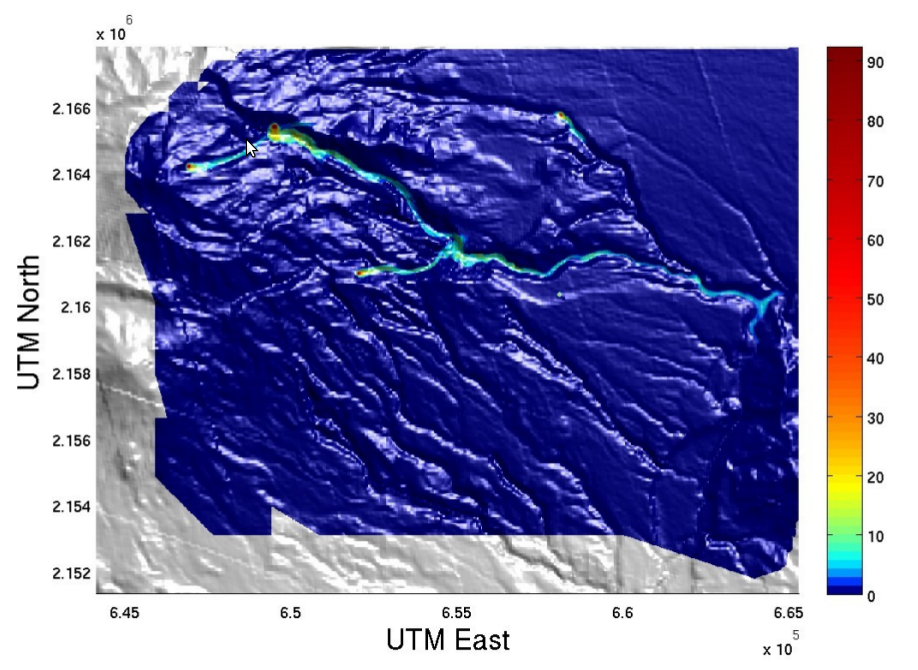
\includegraphics[width=1\textwidth]{IMAGES/rupps1.png}
    \subcaption{ Without thin layer control}
  \end{minipage}
\hspace{0.5cm}
%   \hfill
  \begin{minipage}[b]{.45\linewidth}
    \centering
    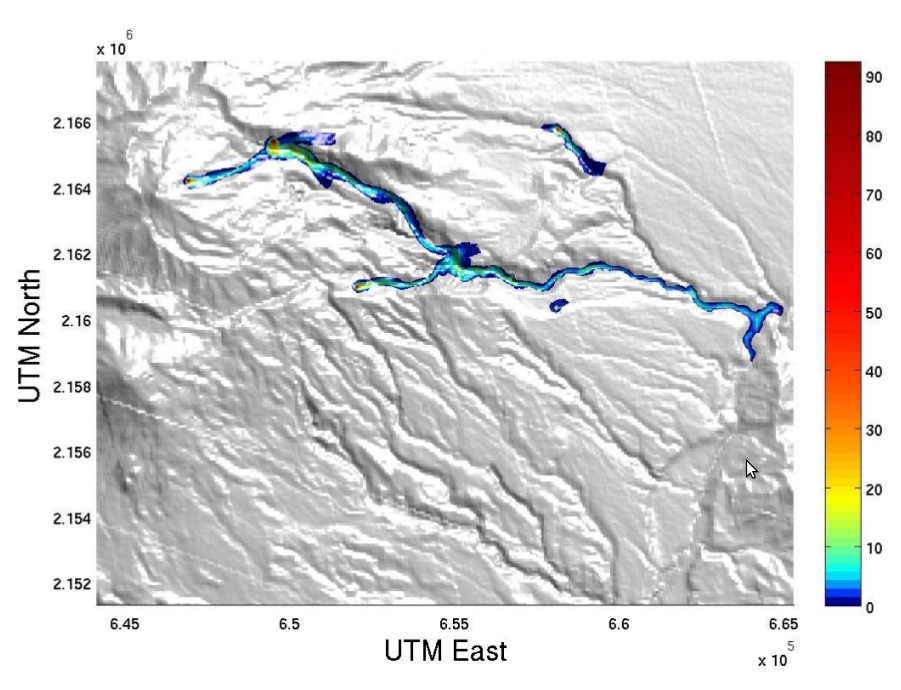
\includegraphics[width=1\textwidth]{IMAGES/rupps2.png}
    \subcaption{Only flow with depth greater than 0.5 m is displayed.}
   \end{minipage}
  \caption{Thin layer problem in maximum over time flow depth simulation of the 1955 debris flow at Atenquique, Mexico \cite{Dalbey2009}.}
  \label{thinlayerproblem}
\end{figure}

Figure \ref{thinlayerproblem} is an example that demonstrate this problem for numerical simulation of granular flow in  Atenquique which is a village near Colima volcano in Mexico. The left figure shows the numerical solution of flow height without using any control for thin layer problem, and the right figure shows the same result with using a naive control with plotting the regions with flow height grater than 0.5 meter. As discussed above, if we do not use any control on the numerical solution, the spread thin layer causes instability and inaccuracy in the obtained results.

% Litrature Review
A review on literature shows numerous attempts were made to overcome this problem over time especially in the recent years \cite{Medeiros2013,Balzano1998,Aureli2008,Bunya2009,Casulli2009a,
Kesserwani2011,DAlpaos2007,Castro2005a}.
Here we will briefly review the topic and refer the interested reader to available references for more information. \newline
Generally, all of the implemented method for the issue could be 
categorized in two basic groups of what we call here heuristic methods and interface tracking/capturing methods.
The basic idea in the first group is to reconstruct the flow interface based upon 
some simple heuristic or some algebraic relations which are not essentially related
to the physics of the problem. In interface tracking/capturing approaches, an auxiliary equation/equations is coupled with the original system of equations in Eulerian or Lagrangian frame of view, to follow the flow interface through its path over time. 
The reason that we mention here both tracking and capturing is that they are usually used for Lagrangian and Eulerian methods respectively.For more information about this group of methods please see \cite{Glimm1995,Unverdi1992,Osher1988,Anderson1998,hirt1981vfv}.\\
In this work to address thin layer problem and other related instability and accuracy problems, we implemented a combination of Heuristic approaches, Phase filed and level set methods and compared the obtained results with experimental and field data for granular flow. Phase field and level set methods are very well-known Eulerian interface capturing methods that to the best knowledge of authors are used for the first time in this application in this work. \newline

%Each of these major groups have their own subcategories which could be found in  
% references, but they will be explained briefly here 
%to provide some insight that is needed in the next parts.\newline
In Heuristic method, the idea is to mitigate thin layer problem with some heuristic strategy. This strategy could be using a threshold to control the thin layer, filling the entire domain with a shallow level of fluid, reconstruction the flow, adjusting the flux, or any combination of them. Most of the attempts that are made to address the thin layer problem are categorized under this sort of method \cite{Aureli2008,Bunya2009,Castro2005a,Kesserwani2011}.

On the other hand, with the interface tracking/capturing methods one can find the interface of a moving boundary flow in a more rigorous way. Based upon the employed frame of work, these methods are divided into Lagrangian and Eulerian methods.
Roughly speaking in Lagrangian type methods, the initial interface is replaced with some of the material points (particles) that represents the interface. These points move with a velocity vector field which comes from numerical solution at each time step. The interface is constructed at each time step by connecting the updated location of these points. 
Mark And Cell (MAC) \cite{Harlow1965}, Simplified Mark And Cell (SMAC)  \cite{Cheng1995}, and Surface Marker \citep{Wrobel1991} methods are some examples of Lagrangian interface tracking techniques.
Obviously, the accuracy of the method is highly depend on the number 
of particles that form the initial boundary. 
High computational cost, tendency to instability and inability to track the complex topological changes are the most important drawbacks of these methods. 
%However, these methods are more useful as an auxiliary tool to compensate the defects of Eulerian methods such as conservation of mass in level set method. 
Tai et el. \cite{Tai2002} is an example of the application of this method for 1D Savage\_Hutter equation. They used a non-oscillatory central (NOC) difference scheme with a stationary uniform mesh, and achieve good results by augmenting this solver with a Lagrangian front tracking scheme.\newline

In the current paper we more focus on interface capturing or Eulerian methods. Level set, phase field and VOF are very well-known methods in Eulerian frame of work.
In these types of methods the interface is captured by solving another transport equation for a scalar that explicitly, in level set method, or implicitly, in VOF and phase field method, indicates the interface location.
This order parameter is coupled with the other governing equations of primitive variables to jointly present a rigorous model for the interested problem.\newline


%%%%%%%%%%%%%%%%%%%%%%%%%%%%%% VOF   %%%%%%%%%%%%%%%%%%%%%%%%%%%%%%%%%%%%%

Hirt and Nichols \cite{hirt1981vfv} were the first to propose a VOF method. 
In this method, the mentioned scalar variable is the fraction/volume of a particular fluid in each cell.
% This equation is material derivative of the scaler variable with respect to the time.
To construct the interface based on this method, the interface surface reconstruction technique shall be performed at each time step. Youngs \cite{youngs1982tdm} achieved a significant improvement in VOF by adding a 
a piecewise linear interface calculation (PLIC) representation of the fluid boundary.  
Youngs' method has been shown to be robust and efficient, but it is only first-order accurate. More advanced methods about this issue are available in \cite{gerlach2006cvf} and Gopala and van Wachem\cite{gopala2008vfm}. 

%%%%%%%%%%%%%%%%%%%%%%%%%% Level set method %%%%%%%%%%%%%%%%%%%%%%%%%%%

Level set method was introduced by Osher and Sethian in 1988 \cite{Osher1988}. In this method, the scalar variable is a signed distance function which shows the distance of each point to the interface. 
%This distance is defined such that is positive for outside of the boundary points and negative for inside of the boundary points. The solution of this equation will show the place of interface at each time step, but since the solution of the original equation is not essentially a signed distance function another equation has to be solved to make the obtained result a signed distance function. This technique is called initialization and re-initialization technique. There are also a number of other methods like fast marching or combination with Lagrangian schemes to get a more accurate result or to get the result with lower computational cost. The main issue about this technique is that, the basic method is not mass conservative and some other complementary methods have to be used to preserve the mass or volume in numerical solution.
The only work that used level set method for WD problem is Quecedo and Pastor \cite{quecedo2002rtg}. They developed Taylor-Galerkin approach to solve the SW equations. They presented two different options for handling the wetting-drying areas. The first approach used was described as a ``simple yet efficient'' method which falls into heuristic method type approaches. Although they claimed that they used level set as the second approach, they did not report any result of that.
They finally concluded that the level set is expensive and unnecessary for their problem.\newline

%%%%%%%%%%%%%%%%%%%%%%%%%% Phse field method %%%%%%%%%%%%%%%%%%%%%%%%%%%

%The last method that we will overview here is phase field method. 
Phase field is another Eulerian interface capturing scheme that the interface is implicitly related to the order parameter which shows the phase variation on the domain \cite{Anderson1998}. In this method the interface is a diffusive region between the phases in spite of level set which yields to a sharp interface. Based on our best knowledge no report was published earlier that uses this method for capturing the interface in SW.
%Usually, this value varies between 0 to 1 or -1 to 1, in such a way that it is 1 if the cell is wet, it is zero (or -1) 
%if the cell is dry, and it has some value between 0 to 1 (or -1 to 1) for partially wet cells.
%This method is more developed and popular in material science research, and drew the attention of the researchers in many disciplines especially in the recent years.
Cahn-Hilliard and Allen-Cahn formulations are two principal formulation for this method \cite{CahnHilliard1958i,CahnHilliard1958ii,Yang2006}. The basic difference between these two form is that the first one is mass conservative, and the second one is not. Mathematically, the conservative form has a forth order derivative while the other one has a second order derivative. This difference in the highest order of derivative will make the later form much easier to implement.\newline
%As a result people first try to use the second one and then if they not succeed, they will proceed to the other one.

%Phase field equation is derived from the relation between the changes of the phases and free energy level of the 
%system. The strong physics behind that makes it powerful particularly in simulating energy and thermodynamics related problems. 

%============= Introduction of next parts of paper =====================
In this paper, we proposed a new multifaceted Heuristic approach and also tested the effectiveness of Level set and Phase field methods to mitigate the thin layer problem difficulties for numerical solution of SW equations. Although these methods have been used for granular type SW flows, most of the conditions holds and the results are applicable for other type of SW flows.  We verified the numerical results with experimental result of a granular SW flow over an inclined plane ends to a horizontal surface , and the field data for Colima volcano.
In Eulerian interface capturing methods we tried to stick to the basic methods, and decrease the computational cost ,when possible, with using some techniques. \newline

%For example, in Level set method we used narrow band re-initialization to just update the value of signed distance function near the interface, and in Phase field we use operator splitting to use implicit solver just for laplacian term and we also used matrix free method to save memory requirement. Detail of these steps can be find in the corresponding section (sections \ref{phase field},\ref{level set}).

In the heuristic approach we first use a very small threshold to discriminate between wet and dry cells, then divide the cells into three groups of wet, dry and partially wet cells. The next step is to adjust the fluxes for the partially wet cells and the last step is to update the state variables for wet cells.\newline

In level set part, we followed the instructions in paper\cite{Sussman} with the re-initialization scheme introduced in Adalsteinsson's work \cite{Adalsteinsson1995}. To solve both of these hyperbolic equations we used a first order accurate solver.\newline

For phase field method, we chose Allen-Cahn formulation. This formulation is not mass conservative. To satisfy mass conservation constrain in this formulation, a Lagrange multiplier is added to RHS of the equation. In this work, we derived a Lagrange multiplier for SW equation. To decrease the computational and memory cost, we used operator splitting and matrix free techniques (detail in section \ref{phase field}). \newline

As a general comparison between the methods it could be mentioned that the first approach is less expensive, but the obtained interface moves a little ahead of the interface found in experimental and field data is. 
On other hand, the interface capturing methods have more strong mathematical and physical structure, and can be coupled with the conversations equations, but are computationally more expensive, and harder to implement.\newline

The structure of the rest of this paper is as follows: in next part SW equations for the geophysical flows and the common features of the solver that we used for all of the three methods are introduced. In section \ref{solution}, 
different methods that were employed to mitigate WD problem are explained. After that the obtained results from the methods are compared, and finally the conclusion of the work is provided.

% =============================================================================
%                METHOD
% =============================================================================
\section{Governing Equations} \label{Method}

% \subsection{SWE for geophysical flows} \label{Governingequations}

The Savage-Hutter equation for geophysical flows was first introduced in the late 1980's. 
Their original model has subsequently been 
improved upon by Savage\_Hutter themselves as well as others  \cite{Hutter1993,Iverson1997,Gray1999,IversonDenlinger2001,PudasainiHutter2003,SavageIverson2003}.
In our earlier work \cite{pitmanpof,gmfg1,dgtitanpaper}, we developed the Titan2D depth-averaged geophysical 
flow simulator.  Titan2D is parallel with dynamic re-partitioning, high order, slope-limiting, upwinding, 
two-dimensional Godunov solver (without splitting), with adaptive mesh refinement and Geographic Information System 
(GIS) integration which lets it use Digital Elevation Models (DEMs) of real terrain.  
While our new multi-faceted thin-layer mitigation strategies were developed in the context of Titan2D's capabilities, 
much of this approach should be appropriate for use in depth-averaged flow solvers with different numerical implementations. \newline
The depth-averaged equations that Titan2D solves are:
\begin{equation} \label{governingeq}
\begin{tabular}{lllllll}
{\Large $\frac{\partial h}{\partial t}$} &+& {\Large $\frac{\partial \left(V_x\cdot h\right)}{\partial x}$} &+& {\Large $\frac{\partial \left(V_y\cdot h\right)}{\partial y}$} &=& $S_h$ \\
{\Large $\frac{\partial hV_x}{\partial t}$} &+& {\Large $\frac{\partial \left(V_x\cdot hV_x+0.5 k_{ap}g_zh^2\right)}{\partial x}$} &+& {\Large $\frac{\partial \left(V_y\cdot hV_x\right)}{\partial y}$} &=&$S_x$ \\
{\Large $\frac{\partial hV_y}{\partial t}$} &+& {\Large $\frac{\partial \left(V_x\cdot hV_y\right)}{\partial x}$}&+& {\Large $\frac{\partial \left(V_y\cdot hV_y+0.5 k_{ap}g_zh^2\right)}{\partial y}$} &=&$S_y$ 
\end{tabular}
\end{equation}

In these equations:
\begin{itemize}
\item The coordinate system (see Figure \ref{xzeast}) is aligned such that $x$ and $y$ are tangential directions 
      to the surface of the 3D terrain and $z$ is normal to the surface.
\item The effect of terrain elevation is represented by gravitational source terms. 
\item $h$ is the flow depth in the $z$ direction that hug the terrain.
\item $hV_x$ and $hV_y$ are the components of ``momentum'' respectively in $x$ and $y$ directions.
\item $k_{ap}$ is a highly nonlinear term that shows the effect of the earth pressure coefficient, which has active 
      (diverging $\mp=-$), passive (converging $\mp=+$), and neutral (neither diverging, nor converging, $k_{ap}=1$) condtions.
\end{itemize}

\begin{equation}
k_{ap}=2\frac{1\mp\sqrt{1-\cos^2(\phi_{int})\left(1+\tan^2(\phi_{bed})\right)}}{\cos^2(\phi_{int})}-1
\end{equation}

\begin{figure}[!t]
\begin{center}
 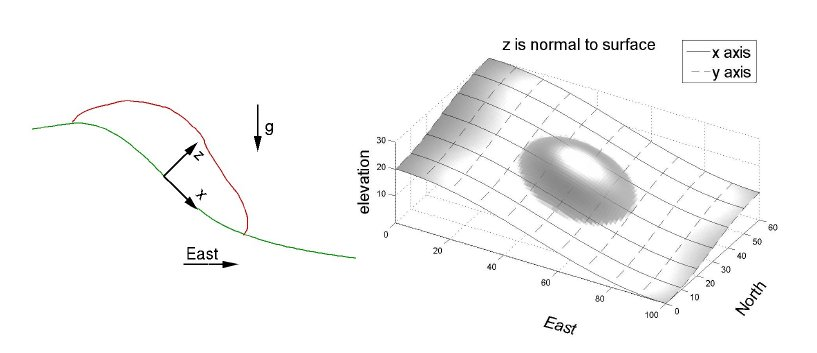
\includegraphics[height=2.8 truein]{IMAGES/1.jpg}
\caption{In the local coordinate system the {\itshape z} direction is normal to the surface; 
the {\itshape x} and {\itshape y} directions are tangential to the surface.}
\label{xzeast}
\end{center}
\end{figure}

Note that in the momentum equations $k_{ap}g_z\frac{h}{2}h$ is the contribution of hydrostatic 
pressure to the momentum fluxes. $S_h$ is a source of mass, i.e. 
material that either effuses or erodes out of the ground. $S_x$ is 
the sum of a gravitational driving force, the friction that resists motion 
of the material relative to the bed, and the friction that resists the 
internal shearing motion of the material see eq. \eqref{momsourceterms}.
\begin{equation}
\begin{aligned}
  S_x &=g_x h - \frac{V_x}{\sqrt{V_x^2+V_y^2}}\max\left(g_z+\frac{V_x^2}{r_x},0\right) h \tan(\phi_{bed}) 
  - {\rm sgn}\left({\frac{\partial V_x}{\partial y}}\right) h k_{ap} \frac{\partial (g_zh)}{\partial y} \sin(\phi_{int}) \\
  S_y &=g_y h - \frac{V_y}{\sqrt{V_x^2+V_y^2}}\max\left(g_z+\frac{V_y^2}{r_y},0\right) h \tan(\phi_{bed}) 
  - {\rm sgn}\left({\frac{\partial V_y}{\partial x}}\right) h k_{ap} \frac{\partial (g_zh)}{\partial x} \sin(\phi_{int}) 
 \end{aligned}
 \label{momsourceterms}
\end{equation}

Titan2D solves the above system of equations with a finite volume Godunov method that is demonstrated in eq. \eqref{integrator}.
\begin{equation}
   \label{integrator}
   U_i^{n+1} = U_i^n - \frac{\bigtriangleup t}{\bigtriangleup x} \{F_{i+\frac{1}{2}}^n - F_{i-\frac{1}{2}}^n \}
   - \frac{\bigtriangleup t}{\bigtriangleup y} \{G_{i+\frac{1}{2}}^n - G_{i-\frac{1}{2}}^n \}
  \end{equation}
  
In the above equation, G and F are the flux terms at the inter-cell boundaries which are computed by HLL Riemann solver that is explained 
in the next section.

\subsection{Using Appropriate Riemann Fluxes} \label{Riemann}
For flux computation TITAN2D uses a HLL solver. HLL solver is an approximate Riemann solver that just use the maximum and 
minimum of characteristic speeds of a hyperbolic system to build the conservative fluxes at the interface.

Following the recommendation of Toro \cite{ToroBook2001}, TITAN2D uses 
the HLL Riemann average of fluxes. Let $U$ be a state variable, $F$ 
be a flux of that state variable, $s$ be a maximum wave speed, 
and $R$ and $L$ subscripts which denote ``right'' and ``left'' values 
respectively.  The HLL Riemann flux is then
\begin{equation}
F_{HLL}=\left\{\begin{tabular}{lll}$F_L$&\hspace{0.5 truein}& if $s_L\ge 0$\\$F_R$&& if $s_R\le 0$\\{\Large 
$\frac{s_RF_L-s_LF_R+s_Ls_R(U_R-U_L)}{s_R-s_L}$}&& otherwise\end{tabular} \right.
\end{equation}
For Savage\_Hutter system of equation the characteristic speeds are: $s_{1,3}=v\pm a$ and $s_2=v$ where $v$ is the 
velocity of fluid in the corresponding direction and $a=\sqrt{k_{ap}gh}$.
But just the above HLL solver is not enough for solving this system of equations.
Fraccarollo and Toro \cite{FraccarolloToro1995} note that at the 
wet-dry boundary the Riemann solution consists of a single rarefaction 
wave whose speed (when averaged over the cell length) 
is bounded above by the cell average flow speed plus 
{\bf twice} the ``speed of sound,'' $s=v+2a$, where $a=\sqrt{k_{ap}gh}$ 
for shallow water type granular flows.  They also note that ``an overestimate 
of the true wave speeds results in enhanced stability'' while an 
``underestimate of the true wave speeds could be fatal'' to stability.
They became the first to 
solve this problem by constructing an approximate Riemann solver.\newline

\subsection{Adaptively Meshing} \label{adaptivemeshing}
In the TITAN2D, each grid cell is square or very nearly so.  Rather than 
using a uniform mesh, different sizes of cells are allowed, with each 
successive ``generation'' covering one fourth the area of its ``parent'' 
cell.  Note that only one generation of irregularity is allowed between 
a cell and its neighbors.\newline

At the beginning of the simulation, i.e. before the first update, the 
boundaries of all piles are maximally refined. An initial mesh for a 
simulation at Colima Volcano, Mexico, is displayed in Figure \ref{bufcell}. 

\begin{figure}[!h]
\begin{center}
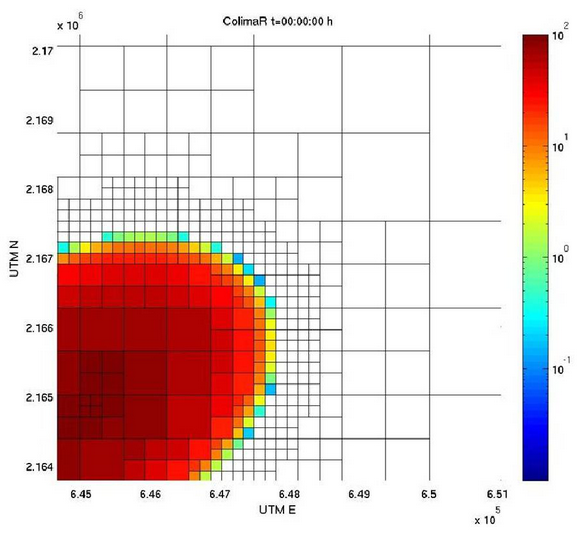
\includegraphics[scale=.3]{IMAGES/buffercells.png}
\caption{Buffer cells}
\label{bufcell}
\end{center}
\end{figure} 

During normal adaptivity, cells are selected for refinement if they meet 
either of two requirements:
\begin{enumerate} 
\item They have large, as compared to the average, inter-cellular fluxes.
\item They are at or within a few cells of any of four small, non-dimensional 
      flow depths (multiples of {\rm\verb1GEOFLOW_TINY1}).
\end{enumerate}
The former condition allows for accurate capture of sharp changes in state 
variables.  The latter results in banded regions of the flow separated into 
``rings'' of maximally refined buffer cells.  This limits artificially high 
transportation of material from the larger depth bands to the lower depth
bands. The outermost ring is at a flow depth of {\rm\verb1GEOFLOW_TINY1}.
The rings are a number of cells wide equal to the number of iterations 
between mesh adaptations.  This guarantees that material will only flow 
into maximally refined dry cells at the wet-dry front.  However, material 
with flow depth less than {\rm\verb1GEOFLOW_TINY1} may be left outside the
outermost band of buffer cells by the passing flow.  The rings of the later  
buffer cells strategy decreases the numerical wicking (Problem 
\ref{problemwicking} from section \ref{introduction}) both within the 
flow and at the boundary.  When combined with thresholding, it is 
sufficient to decrease Problems 
\ref{problemwicking}, \ref{problemtoothin}, and \ref{problemtoofast} to a 
level that prevents the loss of stability due to Problem 
\ref{problemunstable}.\newline

Unrefinement takes place immediately after refinement; a group of four 
``brother'' cells will be selected to merge into their mutual 
``father'' cell if the sum of their inter-cellular fluxes is very low 
compared to the average flux.  Cells that have either just been refined 
or are otherwise in any of the current bands of buffer cells are immune 
to unrefinement.  
    
%     fact that in this paper one of the Eulerian front capturing
% method was used, the advantages and disadvantages of them are provided here.
% The interested reader could refer to \cite{,,,} for more information.

%%%%%%%%%%%%%%%%%%%%%%%%%%%%%%%%%%%%%%%%%%%%VOF%%%%%%%%%%%%%%%%%%%%%%%%%%



% Here we will simply list a few advantages and disadvantages of VOF 
% methods.
% Typically these schemes are only for incompressible fluids, but some 
% work has been done for compressible flows as well.  They are 
% conceptually simple, phenomena like bubble break up and coalescence 
% are included implicitly, and conservation of mass/volume is 
% possible.  However numerical difficulties occur at the interface 
% discontinuity, including difficulty in calculating interface curvature.
% Also, while not an issue for shallow water flows, most volume of fluid 
% methods become complicated in three dimensions. \newline



% %%%%%%%%%%%%%%%%%%%%%%%Phase Field%%%%%%%%%%%%%%%%%%%%%%%%%%%%%%%%%%
% In the phase filed method, the interface is followed 
% implicitly by a continuous order parameter which is called
% here phi. Phi value changes based on the phase variation on the domain. 
% Usually, this value varies between 0 to 1 or -1 to 1, in such a way that if the 
% cell is filled with the fluid phi is one, if it iw partially wet 
% phi is something between (but not equal) 0 to 1 or -1 to 1,
% otherwise the cell is dry and phi is equal to 0 or -1.
% The explained method formes a region that the phase changes smoothly
% from one phase to the other, though the real interface is a sharp line or surface.
% The phase field equation is a PDE that relates the phi to the total free energy, and its solution
% determines the propagation of the discussed variable in the domain. 
% The total energy function is defined regarding to existing 
% variables and the conditions of the under study system.
% Based on the best knowledge of author no report was published
% earlier that use this method for capturing the interface in SWE.

 

\section{Solution}\label{solution}
In the aforementioned parts the major difficulties of numerical analysis of the shallow water
equations were discussed, and it was shown that most of them are directly or indirectly related to the WD problem.
For more intuition, the result of a simulation for Atenquique debris is displayed in figure \ref{thinlayerproblem}. 
The left picture is the obtained result form the solver and the right picture is the same result, but flow height is displayed 
only for flow height greater than 0.5 $m$. This picture shows for the pure solver, that a dominant part of the 
domain is filled with a negligible flow depth and this makes the actual interface mix with the thin layer region, and 
also causes some other problems. In this section, three implemented methods to solve the WD problem which finally yields to 
mitigate the numerical difficulties of SWE are explained. 


\subsection{First: Heuristic method} \label{Heuristic}
All of heuristic methods use one or combination of following four strategies \cite{Medeiros2013}: 
\begin{enumerate}
 
 \item Filling the entire computational domain with a thin layer of fluid
 \item Using a depth scale to check whether a cell or a node is wet or dry 
 (or possibly partially wet), and then  making a decision to add or remove it 
 from the computational domain.
 \item Employing some extrapolating scheme from the wet cells into their neighbor 
 cells to approximate the location of the interface. This method is usually called 
 volume/free-surface relationship (VFR) in the literature.
 \item Permitting fluid height to be negative, which means that it is below the topographical surface.
\end{enumerate}
Each of the above strategies might be more useful for its specific case. Table \ref{table1} compares them very briefly.

\begin{center}\label{table1}
\begin{tabular}{|c|p{5cm}|p{5cm}|}
 
\hline
{\bf Strategy}                  & {\bf Mass Conservation}                                          & {\bf Physics} \\
\hline
{\bf Thin film}                 & Adequate, but requires solution reconstruction 
& Produces a smooth and realistic wetting front     \\
\hline 
{\bf Cell removal}              & Dependent on numerical method for solving the equations          & Excellent, performs better on advancing front than receding front \\
\hline
{\bf VFR}                       & Conservative, with aid of some correction procedure              & Very good in wide verity of problems      \\
\hline
{\bf Allowable negative depth}  & Conservative, but performance depend on WD parameters            & Same as mass conservation      \\
\hline
% \caption{Comparison of different strategies for WD problem in SWE}
\end{tabular}
\end{center}
In this part of the paper the first method that has been used to solve the WD problem in the SWE is explained.
\subsubsection{Selecting appropriate Threshold} \label{Threshold}
In this approach we use a very small threshold to segregate the wet, partially wet and dry cells.
The critical contribution of this scaling is to allow other
facets to identify where the flow %is merely ``thin'' and where it 
is non-physically thin, i.e. where should they consider the boundary of
the flow to be. Consisyency is the key requirement of whatever strategy we choose to
determine the scaling. That is, the
chosen strategy must be able to generate the same ``appropriate'' value
for depth scale at the beginning and at the end of a simulation.  \newline

In a ``typical'' geological simulation, say of the collapse of a volcanic 
dome which would be modeled in TITAN2D as a``pile source,'' the initial 
body of mass can be quite deep, but at the end of the simulation the 
material will likely be spread over a large area.  Hypothetically, if one 
were to scale by maximum flow depth at the beginning and end of the 
simulation, they would obtain vastly different values.  More importantly, 
if the only source of mass was an effusion of material out of the ground, 
the maximum initial flow depth would be zero, even if the total volume 
during the course of the simulation was the same as the previously 
mentioned ``pile source.''  \newline

On the other hand, scaling by the cube root of the total volume of the 
flow being simulated is entirely consistent and is the flow depth 
scaling factor used by TITAN2D.  We do {\bf not} claim that the cube root 
of volume is any more or less appropriate as a scaling factor than 
maximum initial flow depth in other shallow water contexts, for example 
storm surge simulation.\newline

Having chosen a consistent scaling factor, we were then able to define 
associated non-dimensional depths for negligibly thin and merely thin
flow.  If one were to assume that a particular geophysical mass flow 
event involved a volume of $10^8 [{\rm m}^3]$, it would then be 
reasonable to state that flow depths of less than $5 [{\rm cm}]$ were
both negligible and non-threatening.  This roughly equates to 
non-dimensional negligible flow depth, which we call 
{\rm\verb1GEOFLOW_TINY1}, with the value 
\begin{equation}
{\rm\verb1GEOFLOW_TINY1} = 0.0001
\end{equation}
Using this value, and assuming
the volume used in a laboratory scale test was $1 [{\rm cm}^3]$, the 
resultant negligible flow depth would be $0.0001 [{\rm cm}]$.  As can 
be observed from these two examples, the chosen value of 
{\rm\verb1GEOFLOW_TINY1} is physically appropriate across a very large 
range of volumes.  We therefore use a theoretical contour at this depth 
as the boundary of the simulated flow.  %\newline

%     \subsubsection{Thresholding} \label{thresholding}
In introduction section we stated that, unless steps are taken to 
prevent it, the numerical wicking (Problem \ref{problemwicking}) will
cause the flow to spread 1 cell every time-step even though the product
of flow speed and time-step size is less than the cell length.  In 
addition, the familiar continuum equations loose hyperbolicity (wave 
speeds tend to infinity) at the boundary between a continuous material 
and a vacuum.  Having implicitly defined the flow boundary,
we prevent calculation of state variables outside the flow, i.e. in 
regions with flow depth below {\rm\verb1GEOFLOW_TINY1}.  
This reduces both non-physical flow 
spreading and computational cost. Note that state variables in cells 
with flow depth less than {\rm\verb1GEOFLOW_TINY1} are {\bf not} zeroed.  \newline

% Once having made the the decision to implement the negligible flow 
% depth threshold, one is faced with choosing a value for the threshold.
% If the chosen threshold is overly large, it would impose a non-physical 
% limit to the flow.  Consequently, the previously stated value of 
% {\rm\verb1GEOFLOW_TINY1} was chosen with the intention of being 
% conservatively low.  However, this results in the negligible flow 
% depth threshold not being able to entirely circumvent the loss of 
% hyperbolicity (Problem \ref{problemunstableB} from Subsection 
% \ref{CausesSubSec}).  We compensate for this through appropriate Riemann 
% fluxes. Thresholding also decreases the numerical wicking (Problem 
% \ref{problemwicking}) at the flow boundary.




\subsubsection{Interface Reconstruction} \label{Interfacerecon}
As noted above, the use of a standard Eulerian grid imposes discrete 
fixed increments to flow extent, which contributes to the wicking problem
(Problem \ref{problemwicking} ) at the 
boundary.  Use of adaptive mesh refinement 
reduces this error by reducing the size of the increment where it is
most beneficial to do so.  The Lagrangian approach does not have this 
limitation, which Tai et al. \cite{Tai2002} took advantage
of when they augmented their one dimensional NOC scheme with 
Lagrangian front tracking.  However, implementing a hybrid 
Eulerian-Lagrangian scheme in two dimensions is significantly more 
complex.  \newline

Therefore as part of our multi-faceted approach, we implemented a very 
simple and inexpensive interface reconstruction and predictive 
Lagrangian front tracking scheme.  Knowledge of the interface allows
us to generate more a representative average, for an individual cell edge 
over the time-step, and for values of state variables which are then used to 
compute inter-cellular fluxes into/out-of partially wet cells.  The 
interface reconstruction scheme is illustrated in figure \ref{interface}.\newline

\begin{figure}[!h]
\centerline{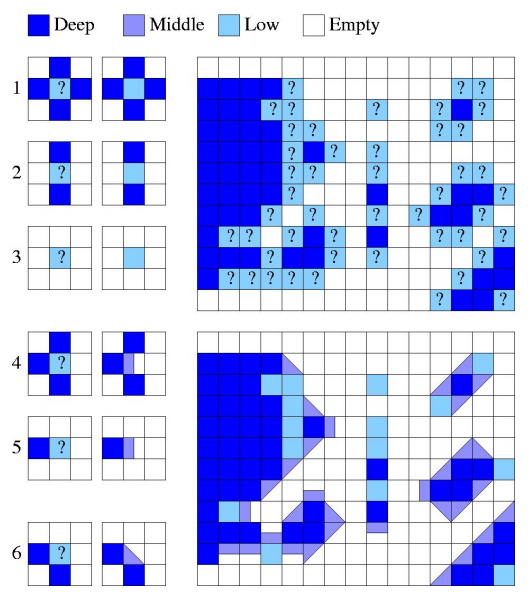
\includegraphics[scale=0.3]{IMAGES/flux.png}}
\caption{Interface Reconstruction in TITAN2D}
\label{interface}
\end{figure} 
%\clearpage

Specifically, each partially wet cell is assumed to be split by a 
straight line into a completely dry and a completely wet part.  For the 
sake of simplicity, we restrict this line to one of four orientations: 
east-west, north-south, or parallel to either diagonal of the square
cell.  However, all placements/translations of the wet-dry line are 
allowed.  At the beginning of each time-step, the orientation of the 
line for the entire time-step is set based solely on which of the cell's 
neighbors have flow depth greater/less than the {\rm \verb1GEOFLOW_TINY1} 
threshold\footnote{As stated in Subsection \ref{adaptivemeshing}, the 
refinement strategy ensures that the flow front will always be maximally 
refined.  This  simplifies the coding since all cells at the front can be
safely assumed to have only one neighbor on each side.}.   Orientation
of the wet-dry line, and which side of it is wet, is indicated by a single 
integer representing the geometrically determined ``most wet node.'' 
The only nine possible values for the most wet node are be any of the 
cell's corners, edge midpoints or its center.  The most wet node is 
assumed to have a flow depth that is the maximum of the cell or any of 
its four neighbors.  The placement of the line is such that the volume of 
material in the cell under a plane passing through the most wet node
and the wet dry-line is the same as the unadjusted cell.\newline  %Knowing the 
%wet-dry line's placement, the wet part only average of a conservative 
%state variables equals its whole cell average value divided by the 
%fraction of the cell's area that is wet.

Since we now know where the wet-dry line is at the beginning of the 
time step, we can compute which of the cell's edges are completely 
wet, completely dry, or partially wet, and the fraction of wetness for 
the partially wet edges.  Given the orientation and beginning of 
time-step location of the wet-dry line and the cell's state variables, 
it is also fairly straight forward to predict the line's end of 
time-step location.  This is done by convecting the wet-dry line at 
the shock speed, $s=v+a$ where the speed of sound has been adjusted 
to account for only part of the cell being wet, i.e. 
$a=\sqrt{k_{ap}gh\frac{A}{A_{wet}}}$.  Here $A$ is the whole cell's 
area and $A_{wet}$ is the portion of the cell's area that is wet.  \newline

Since the wet-dry boundary within each partially wet cell is assumed 
to be a straight line width, during the time-step, fixed orientation, 
convecting a single point, in this case the midpoint, on the line is 
equivalent to convecting the entire wet-dry line.  A spatial and time 
average of the wetness factor for the edge over the time-step can 
therefore be easily computed as
\begin{equation}
W=\left(\frac{0\cdot\Delta t_{dry} +\frac{1}{2}(w_{beg}+w_{end})\Delta t_{part}+1\cdot\Delta t_{wet}}{\Delta t}\right) \left(\frac{A}{A_{wet}}\right)
\label{wetnessfactor}
\end{equation}
Where $\Delta t=\Delta t_{dry}+\Delta t_{part}+\Delta t_{wet}$ is the 
entire time-step, $\Delta t_{dry}$ is the portion of the time-step for 
which the edge is completely dry, $\Delta t_{part}$ is the portion of 
the time-step for which the edge is partially wet and partially dry, 
$\Delta t_{wet}$ is the portion of the time-step for which the edge is 
completely wet, $w_{beg}$ is the edge's fraction of wetness at the 
beginning of the time-step, and $w_{end}$ is the edge's fraction of 
wetness at the end of the time-step.\newline

\subsubsection{Adjusting Fluxes in Partially Wet Cells} \label{adjustfluxes}

The state variables used to compute the physical fluxes are the whole
cell average values multiplied by the edge wetness factor.  Note this 
results in the zeroing of this cell's physical fluxes for its sides 
that will be completely dry for the entire time-step and increasing 
them for sides that will be completely wet for the entire time-step.   
The numerical fluxes are then taken to be the HLL Riemann average of 
the ``adjusted'' physical fluxes from the cells on both sides the edge.  \newline

The wetness factor adjustment of fluxes delays/decreases the transfer 
of material from partially wet cells to completely dry cells.  This 
delay significantly reduces the amount of non-physical flow spreading, 
and requires negligible additional computation and memory usage.  In 
terms of memory usage, this scheme only requires one additional
integer indicating the most wet node, and two additional decimal 
numbers for the cell's fraction of wet area and the location of the 
wet-dry line's midpoint (implemented as a single number ranging from 
zero to one).  The flux adjustment in partially wet cells mitigates
the numerical wicking (Problem \ref{problemwicking}) at the boundary but not within the flow (that
requires either a uniform grid or an adaptive strategy based on
fluxes and the rings of buffer cells strategy).
% 
% {\bf 1D Analysis of partially wet flux adjustment}\newline
% 
% There are 3 cells L, M, R.  $h_R=V_R=0$, $h_L>2 h_M>0$ (the middle cell is partially wet), $V_L>0$, $V_M>0$.  The timestep is set by the middle cell with a Courant number $C$. \newline
% 
% The wet area of the {\it partially wet} middle cell is defined as follows
% \begin{eqnarray}
% h_m A &=& \frac{1}{2} h_L A_wet  \\
% \frac{A_{wet}}{A} &=& 2\frac{h_m}{h_L}
% \end{eqnarray}
% More generally 
% \begin{equation}
% \frac{A_{wet}}{A}=\min\left(1,2\frac{h_m}{h_L}\right)
% \end{equation}
% We can then compute a wet portion average of $h$ and $hV$ for the middle cell
% \begin{eqnarray}
% \hat{h}_m&=&h_m\frac{A}{A_{wet}} \\
% \widehat{(hV)}_m &=& hV\frac{A}{A_{wet}}
% \end{eqnarray}
% The adjusted wave speeds in the middle cell are $s=V_m \pm 2\alpha\sqrt{\hat{h}_m}=V_m \pm 2 \alpha \sqrt{h_m} \sqrt{\frac{A}{A_{wet}}}$.  This makes the timestep
% \begin{equation}
% \Delta t = C \frac{\Delta X_m}{V_m+2\alpha\sqrt{h}\sqrt{\frac{A}{A_{wet}}}}
% \end{equation}
% The wet-dry line can then be convected at $s=V_m+2\alpha\sqrt{h_m}\sqrt{\frac{A}{A_{wet}}}$ and the time at which the flow will reach the edge of middle and right cells.   
% \begin{eqnarray}
% \Delta t_{part} &=& \min\left(\Delta t, \frac{\Delta X_m \left(1-\frac{A_{wet}}{A}\right)} {V_m+2\alpha\sqrt{h}\sqrt{\frac{A}{A_{wet}}}}\right) \\
% \Delta t_{wet}&=&\Delta t - \Delta t_{part} 
% \end{eqnarray}
% We can then define a time averaged wetness factor, $W_{MR}$ for the middle cell for the edge shared by the middle and right cells
% \begin{eqnarray}
% W_{MR}&=&\frac{\Delta t_{wet}}{\Delta t} \frac{A}{A_{wet}}\\
% &=&\left(1-\frac{\Delta t_{part}}{\Delta t}\right)\frac{A}{A_{wet}}\\
% &=&\frac{A}{A_{wet}}-\min\left(\frac{A}{A_{wet}},\frac{\frac{\Delta X_m}{\Delta t} \left(\frac{A}{A_{wet}}-1\right)}{V_m+2\alpha\sqrt{h}\sqrt{\frac{A}{A_{wet}}}}\right)\\
% W_{MR}&=&\frac{A}{A_{wet}}-\min\left(\frac{A}{A_{wet}},\frac{1}{C}\left(\frac{A}{A_{wet}}-1\right)\right)
% \end{eqnarray}
% Then 
% \begin{eqnarray}
% F_{hMR}^*&=&\frac{\left(V_m+2\alpha\sqrt{h_m}\sqrt{\frac{A}{A_{wet}}}\right)W_{MR}h_mV_m-\left(V_m^2-4\alpha h_m\frac{A}{A_{wet}}\right)W_{MR}h_m}{4\alpha\sqrt{h_m}\sqrt{\frac{A}{A_{wet}}}}\\
% &=&\frac{W_{MR}h_m}{2}\left(V_m+2\alpha\sqrt{h}\sqrt{\frac{A}{A_{wet}}}\right)
% \end{eqnarray}
% Likewise 
% \begin{eqnarray}
% F_{hVMR}^*&=&\frac{\left(V_m+2\alpha\sqrt{h_m}\sqrt{\frac{A}{A_{wet}}}\right)\left(W_{MR}h_mV_m^2+\frac{1}{2}\alpha^2W_{MR}^2h_m^2\right)-\left(V_m^2-4\alpha h_m\frac{A}{A_{wet}}\right)W_{MR}h_mV_m}{4\alpha\sqrt{h_m}\sqrt{\frac{A}{A_{wet}}}}\\
% &=&...
% \end{eqnarray}
% 
% The middle cell's wetness factor, $W_{ML}$, for the edge shared with the left cell is
% \begin{equation}
% W_{ML}=\frac{A}{A_{wet}}
% \end{equation}
% Note that if the wet-dry line does not reach the edge shared by the middle and right cells within the timestep then $W_{MR}=0$.  Assuming that this is the case then
% $h_R'=V_R'=0$ and ... \newline
% $h_M'$, and $V_M'$ also depend on $h_L$ and $V_L$ so their values must be known/assumed in order to compute/simplify $h_M'$ and $V_M'$

\subsection{Second: Phase Field Method} \label{phase field}
As noted earlier, the other approach that is employed 
for capturing the interface of a SW type flow is phase field method.
In this method, a continuous
order parameter is augmented into the state variables. This order parameter that is displayed here with $\varphi$, 
implicitly represent the interface in the domain. To this aim, a new transfer equation must be solved which is coupled with the other state variables. Papers \cite{Chen2002,Anderson1998,Boettinger2002,Kim2012} are good references about the history and evolution of the method.\\
Phase diffusion methods and particularly phase field method is base upon the notion that the interface between phases is a diffusive region rather than a sharp interface with a finite width. 
Value of $\phi$ is constant inside the bulk phases but changes smoothly between the phases. In this work $\phi$ is 1 for the fluid phase $ \lbrace \textbf{x}, \phi(\textbf{x},t)=1 \rbrace  $, and it is -1 for void regions $ \lbrace \textbf{x}, \phi(\textbf{x},t)=-1 \rbrace  $, and is between -1 to 1 on the diffusion region $ \lbrace \textbf{x}, -1 < \phi(\textbf{x},t) < 1 \rbrace  $. Then we can implicitly assume the interface of flow is where $ \lbrace \textbf{x}, \phi(\textbf{x},t)= 0 \rbrace  $.\newline

%The strong thermodynamical and physical derivation of the method make it so powerful for capturing the complicated topological changes especially for the problems that the interface motion depends on gradients of an external field normal to the interface and on the local curvature of the interface.
Cahn-Hilliard and Allen-Cahn are the two principal phase field formulations. Basically, Cahn-Hilliard and Allen-Cahn are two possible gradient flows that can describe the phase diffusion. Both of the formulation can be written in the form of equation \eqref{generalphase}. 
% that are displayed in eq. \eqref{cahnhilliard} and eq. \eqref{allencahn} respectively.
% The derivation of the equations in more detail could be found in \cite{CahnHilliard1958i,CahnHilliard1958ii}. 
 As could be seen, the time material derivative of $\varphi$ is related to the gradient of a energy functional. For Allen-Cahn formulation, this energy functional is Ginzburg-Landu \eqref{ginzlandu}. 
The basic difference between this formulations is that
Cahn-Hilliard is mass conservative but Allen-Cahn is not. From computational point of view, there is a bi-harmonic term in the right hand side of Cahn-Hilliard equation which is forth order derivative and makes computationally expensive to implement. Usually, people try to 
use Allen-Cahn first and then if the result was not satisfactory they switch to Cahn-Hilliard phase field. 
Since in our work we intend to find the interface with the least computational cost Allen-Cahn form was chosen. 

\begin{equation}
 \label{generalphase}
\frac{D \varphi }{D t} = - \frac{\gamma}{\eta} \frac{\delta W} {\delta \varphi} 
\end{equation}

\begin{equation}
 \label{ginzlandu}
 W(\varphi,\nabla \varphi) = \int_\Omega \lbrace\frac{\eta}{2} |\nabla \varphi|^2 + F(\varphi) \rbrace dx
\end{equation}

%\begin{equation}
% \label{generalphase}
%\frac{\partial \varphi }{\partial t} + \overrightarrow{V} \cdot \bigtriangledown \varphi = 
%\bigtriangledown \cdot (M(\varphi) \bigtriangledown\mu(\varphi)))
%\end{equation}
%which \newline
%\begin{equation}
%\mu = F'(\varphi)- \varepsilon^2 \Delta (\varphi)
%\end{equation}
In equation \eqref{generalphase}, $ \eta $ is a constant that regulates the capillary width or diffusion width, and $ \gamma $ denotes elastic relaxation constant. In our case, we select:
\begin{equation}
 \label{freeenergy}
  F(\varphi)=\frac{1}{4\eta} (\varphi^2-1)^2 ,
  \end{equation}
which is the well-known double-well potential function, and represents the interactions of different volume fractions of individual species. The gradient part $ \frac{\eta}{2} |\nabla \varphi|^2  $, is the relaxtion part that relates the the mass average of the energy, with the volume average of the elastic energy \cite{Bronsard1990,Larson1999}.
Putting \eqref{freeenergy} in to equation \eqref{generalphase} leads to: 
\begin{equation} 
\label{allencahn}
\frac{\partial \varphi }{\partial t} + \overrightarrow{V}\cdot \nabla \varphi = 
\gamma (\bigtriangleup\varphi -F'(\varphi)+\xi(t)),
\end{equation}

where

\begin{equation} 
\label{fprime}
F'(\varphi)= \frac{\delta F}{\delta \varphi} = \frac{1}{\eta} \varphi (\varphi^2 -1).
\end{equation}
As discussed before, the Allen-Cahn formulation is not mass conservative, so to conserve the mass a Lagrange multiplier is added into 
the equation as a source term that is displayed in equation \eqref{allencahn} by $\xi(t)$. In our case, we have an initialie pile of volcaninc flow that hat be constant during the all simulation, so the constrain that we want to be satisfied is:
\begin{equation} 
\label{constrain}
\frac{D}{Dt} \int_\Omega \varphi h \ \ dx= 0.
\end{equation}
The reason that equation \eqref{constrain} holds is that we selected $ \lbrace \textbf{x}, \phi(\textbf{x},t)= 1 \rbrace  $ for the regions that granular material exist. Thus, the result of integral is nothing else than the initial volume of pile that has to be fix for all simulation time. This constrain is different with the constrain that usually is used to conserve the mass in Allen-Cahn formulation, and we have to find a new $\xi(t)$. The detail of derivation is in Appendix \ref{app1}, and the result of that is shown in \eqref{xit}.

\begin{equation} 
\label{xit}
\xi(t) = \frac{1}{V_0} \int_\Omega\  h F'(\varphi) \ dx
\end{equation}
 
where  $ V_0 $ is the initial volume of the pile.
In all of our simulation we used $\eta=4\delta x$, where $\delta x$ is equal to the smallest cell length. Since we use the result of phase field for mesh refinement, and we always have the smallest cell size near the interface, using this $\eta$ means that we select the length of capillary width to be equal to size of four cells.
% 
% \begin{equation}
% F(\varphi) =  0.25 \varphi^2 (\varphi -1)^2 
% \end{equation}

%Depending on the problem conditions there are different choices for the mobility function, such as $M(\varphi)=1-\varphi^2$ or $M(\varphi)=1$ \cite{}. For this work we selected the later one.\newline
% \[ \large \frac{d}{dt} \int_X \varphi \, dx = 0 \]
% In the above equation \xi(t) is the Lagrangian multiplier 
% to constrain the volume constant.
The default time integration scheme in TITAN2D is forward Eulerian scheme. This scheme is less expensive and fast but conditionally 
stable. Satisfaction of CFL condition is the necessary condition for stability in this scheme. Since phase field 
method has a second order derivative, to satisfy CFL condition which in this case is related to the inverse square of the spatial increment, CFL $\propto \bigtriangleup \text{x}^{-2}$, thus time increment must be proportional to the square 
of the spatial increment, $\bigtriangleup \text{t} \propto ( \bigtriangleup x)^2 $, makes the time step too small and causes unaffordable simulation time.
Thus the time integration scheme must be changed to another time scheme which allows larger time steps.
The Eulerian implicit time scheme is unconditionally stable, but the disadvantage of this method is a system of linear equations has to be solved at each time step which impose a high computational cost.
To overcome this problem we used operator splitting method to either make the time scheme stable for larger time steps, and maintain the computational cost low.  
By the operator splitting scheme that we used here the time integration of laplacian term is performed with Eulerian implicit scheme and the rest of terms are updated in the explicit time integrator. This solution let us to select larger time steps for implicit solver, let say for example quadruple of explicit time step, and consequently the system of equations has not to be solved at each time step. However because the solver needs to know for what cells the state variables have to be updated, the solution of the phase field is required at each time step. Therefore an extrapolation (or prediction step) based on the Taylor series was computed for intermediate time steps to approximate the phase field solution between the implicit solver time steps.
This is basically a predictor-corrector scheme which is used broadly for advection-diffusion equations solvers. Equations \eqref{implcit_phi}, and  \eqref{explicit_phi} are respectively implicit and explicit time integrators.\\
%, and 
%figure \ref{figintegrator} shows the operator splitting time integration schematically.\\

% 
% \begin{equation}
% \label{operator splitting}
% \large \frac{\partial \varphi}{\partial t} = \frac{\partial \varphi_1}{\partial t} + \frac{\partial \varphi_2}{\partial t} 
% \end{equation}

\begin{table*}[h]
\noindent\begin{minipage}[b]{.5\textwidth}
    \begin{align}\label{explicit_phi}
\frac{\partial \varphi_1}{\partial t} + \overrightarrow{V} \cdot \triangledown \varphi_1 &= f(\varphi_1) \notag \\
 L_1 &= V_x \frac{\partial }{\partial x} + V_y \frac{\partial }{\partial y} \notag \\
\frac{\varphi_{1}^{n+1}-\varphi_{1}^{n}}{\triangledown t} &= f(\varphi_{1}^{n}) - L_1 \varphi_{1}^{n} \notag \\
\varphi_{1}^{n+1} &= \triangledown t \  ( f(\varphi_{1}^{n}) - L_1 \varphi_{1}^{n}) 
\end{align} 
\end{minipage}%
\begin{minipage}[b]{.5\textwidth}
    \begin{align}\label{implcit_phi}
\frac{\partial \varphi_2}{\partial t} &= \alpha \triangledown^2 \varphi_2 \notag \\
L_2 &= \alpha (\frac{\partial^2 }{\partial x^2} + \frac{\partial^2 }{\partial y^2}) \notag  \\
\displaystyle \frac{\varphi_{1}^{n+1}-\varphi_{1}^{n}}{\triangledown t} &= \alpha L_2 \varphi_{2}^{n+1} \notag \\
( 1- \triangledown t \alpha L_2 ) \varphi_{1}^{n+1} &= \varphi_{2}^{n}
\end{align} 
\end{minipage}
%\caption{Left column is explicit time integrator, and right column is implicit time integrator}
\end{table*}




%\begin{figure}[!h]
%
%\begin{center} 
%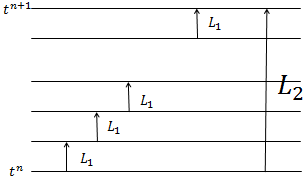
\includegraphics[width=2.5truein]{IMAGES/integrator.png}
%\caption{This picture displays the schematic time integration scheme }
%\label{figintegrator}
%\end{center}%
%\end{figure}
To preserve the scalability of TITAN2D, for solving the equations we used PETSc \cite{petsc-user-ref} library. GMRES solver which is a iterative Krylov subspace solver 
was exploited to solve the system of equations. To decrease the memory cost, we used matrix-free method to compute the laplacian term.
Since the Krylov subspace solvers just need the result of matrix-vector multiplication instead of an explicit definition of matrix 
of coefficients, matrix-free method can be used to get the result of this multiplication by doing some algebraic operation on 
the participant vector in the production. This method leads to a significant saving in required memory cost.

\subsection{Third: Level Set Method} \label{level set}

The last test method for tracking the interface for a SW flow is the Level set method.
Level set method is another Eulerian interface capturig method that was introduced by Osher and Sethian in 1988 \cite{Osher1988}.
The basic of the method is to capture the interface by means of solving a hyperbolic Hamilton-Jacobi PDE on 
the computational domain which follows the evaluating of the boundaries. The level set variable $\varPsi (X,t)$ explicitly 
represents the interface. In this method, $\varPsi (X,t)$ is defined such that its value is zero on the interface, and 
changes in the domain with respect to the distance of each point to the zero level set or interface of the flow. 
In other words, $\varPsi (X,t)$  is a distance function, so that its value is negative for the points inside the boundaries, 
positive for points outside of the boundary, and is zero on the interface. 
This method is not originally mass conservative, but with doing some 
techniques like fast reinitialization mass conservation could be achieved. 
To derive the level set equation, given the initial location of the boundary an initial signed distance function on 
the domain which could be found by the initialization techniques that will be discussed later. The evolution of initial 
boundary in a moving continuum Eulerian frame of work only depends on the normal velocity of the boundary $F$, 
and the tangential velocity does not cause any topological change. Consequently, the following equation could 
be written for the $\varPsi (X,t)$ :

\begin{equation}\label{levelseteq1}
 \frac{\partial \varPsi}{\partial t} + F |\bigtriangledown \varPsi| = 0
\end{equation}

Substituting $F = \overrightarrow{V} \overrightarrow{n} $, and 
$\overrightarrow{n} = \frac{\bigtriangledown \varPsi}{|\bigtriangledown \varPsi|}$
relations into eq. \eqref{levelseteq1} leads to \eqref{levelseteq2}

\begin{equation}\label{levelseteq2}
 \frac{\partial \varPsi}{\partial t} + \overrightarrow{V} \bigtriangledown \varPsi = 0
\end{equation}

Equation \eqref{levelseteq2} is a non-conservative hyperbolic equation. We used a first order upwind scheme  that is explained in detail in \cite{} to solve this equation. 

\begin{equation}
   \label{explicit}
   U_i^{n+1} = U_i^n - \frac{\bigtriangleup t}{\bigtriangleup x} \{F_{i+\frac{1}{2}}^- + F_{i-\frac{1}{2}}^+ \}
   - \frac{\bigtriangleup t}{\bigtriangleup y} \{G_{i+\frac{1}{2}}^- + G_{i-\frac{1}{2}}^+ \}
  \end{equation}
Where $F$ and $G$ are the flux terms and are coming from the flux term for in upwind scheme:


% \[ F_{i+\frac{1}{2}}^- = \left\{ \begin{array}{ll}
%          \mathop{\mathlarger{\frac{v_r+v_l}{2}(v_r-v_l)}} \ \ \ \ \   & \  \\
%          \ \ &\ v_l < 0 \\
%          0 \ \ \ \ \   & \   .\end{array} \right. \] 
% 
% and 
% 
% \[ F_{i+\frac{1}{2}}^+ = \left\{ \begin{array}{ll}
%          0 \ \ \ \ \   & \  \\
%          \ & \ v_l > 0\\
%          \mathop{\mathlarger{\frac{v_r+v_l}{2}(v_r-v_l)}} \ \ \ \ \   & \ .\end{array} \right. \] 
         
% same formulation can be used to find G fluxes.

\subsubsection{Reinitialization} \label{reinitialization}

To generate the initial signed distance function in the beginning and also to keep the solution of the level set equation during 
the time, we need a procedure that is called initialization or reinitialization. There are several techniques to make the obtained 
solution a signed distance function \cite{Osher1988}, but what we implemented here is the method presented by 
Sussman et al \cite{Sussman}. In this reinitialization technique another hyperbolic equation is solved to adjust the $\varPsi$ value 
in the domain:

\begin{equation}\label{initializationeq}
 \frac{\partial \varPsi}{\partial \tau} + sign(\varPsi) (|\bigtriangledown \varPsi| - 1)= 0 
\end{equation}

In eq. \eqref{initializationeq} $\tau$ is a pseudo-time and the equation should be solved until it converges reasonably. 
As it is clear from the equation the result of this equation does not change the zero level set, but it adjusts the other level sets 
in a sense that $|\bigtriangledown \varPsi|=1$.
The method that introduced by \cite{Adalsteinsson1999} was used to obtain the solution of re-initialization equation. Since the re-initialization 
is not required for every time step, the re-initialization was performed after every five time steps.

\begin{equation}
 \varPsi_{ijk}^{n+1}=\varPsi_{ijk}^{n}-\bigtriangleup t \left(max(F,0)\bigtriangledown_{ijk}^{+}+min(F,0)\bigtriangledown_{ijk}^{-} \right),
\end{equation}

where 

\begin{equation}
\begin{aligned}
 \bigtriangledown_{ijk}^{+} = \big[ & max(D^{-x}\varPsi_{ijk}^{n})^2 + min(D^{+x}\varPsi_{ijk}^{n})^2
 \\& max(D^{-y}\varPsi_{ijk}^{n})^2 + min(D^{+y}\varPsi_{ijk}^{n})^2 \big]^{1/2}
\end{aligned}
\end{equation}
 
\begin{equation}
\begin{aligned}
 \bigtriangledown_{ijk}^{-} = \big[ & min(D^{-x}\varPsi_{ijk}^{n})^2 + max(D^{+x}\varPsi_{ijk}^{n})^2
 \\& min(D^{-y}\varPsi_{ijk}^{n})^2 + max(D^{+y}\varPsi_{ijk}^{n})^2 \big]^{1/2}
\end{aligned}
\end{equation} 

In the above equations $D^+$, and $D^-$ are  respectively the backward and forward differences in the corresponding directions.


\section{Results} \label{results}
\subsection{Inclined plane}
In this section the results of the study is presented in the same order they were introduced in the paper.
Table 1 shows the applied initial condition for these results.
\begin{center}
 
\begin{tabular}{|l|c|}

% \caption{Initial condition}
\hline
Maximum pile height       & .06 m \\
\hline
Major extent of the pile  & .06 m \\
\hline
Minor extent of the pile  & .06 m \\
\hline           
Bed friction angle        & $32.47^o$ \\
\hline
Initial friction angle    & $37.3^o$ \\
% \hline
% Initial velocity          & 2 m/s \\
\hline
\end{tabular}
\end{center}


\begin{figure}[H]
  \begin{minipage}[b]{.48\linewidth}
    \centering
    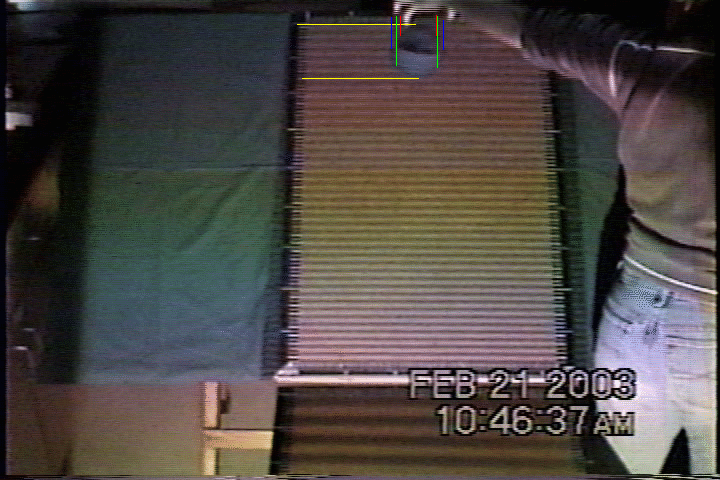
\includegraphics[width=1\textwidth]{IMAGES/expinitialconf.png}
    \subcaption{Experimental setup}
  \end{minipage}
%   \hfill
  \begin{minipage}[b]{.48 \linewidth}
    \centering
    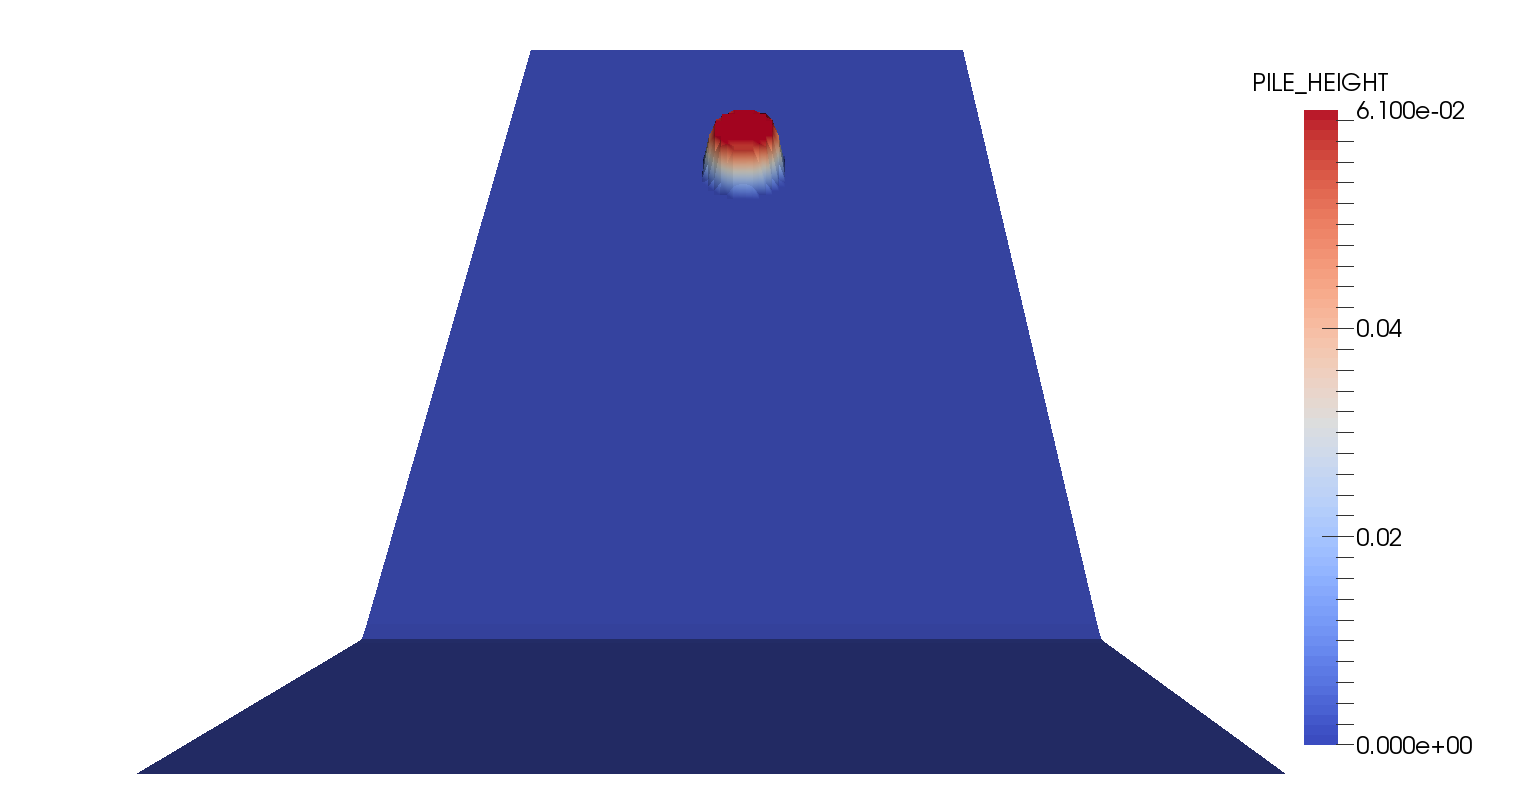
\includegraphics[width=1\textwidth]{IMAGES/initialconf.png}
    \subcaption{Numerical simulation}
  \end{minipage}
  \caption{Initial configuration of the pile on the incline}
  \label{initialconf}
\end{figure}


%\subsubsection{Heuristic Method}

\begin{figure}[H]
  \begin{minipage}[b]{.48\linewidth}
    \centering
    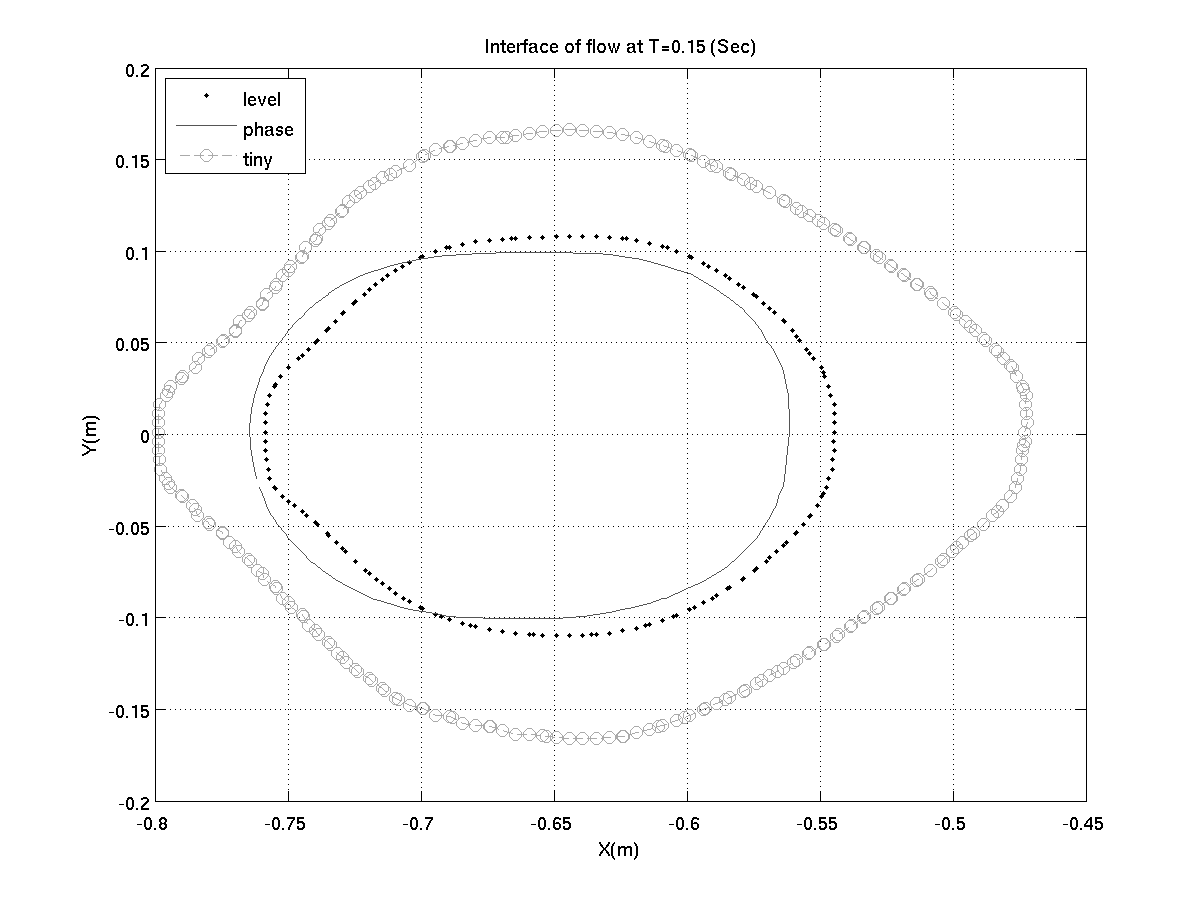
\includegraphics[width=1\textwidth]{IMAGES/interface15.png}
    \subcaption{T=0.15 sec}
    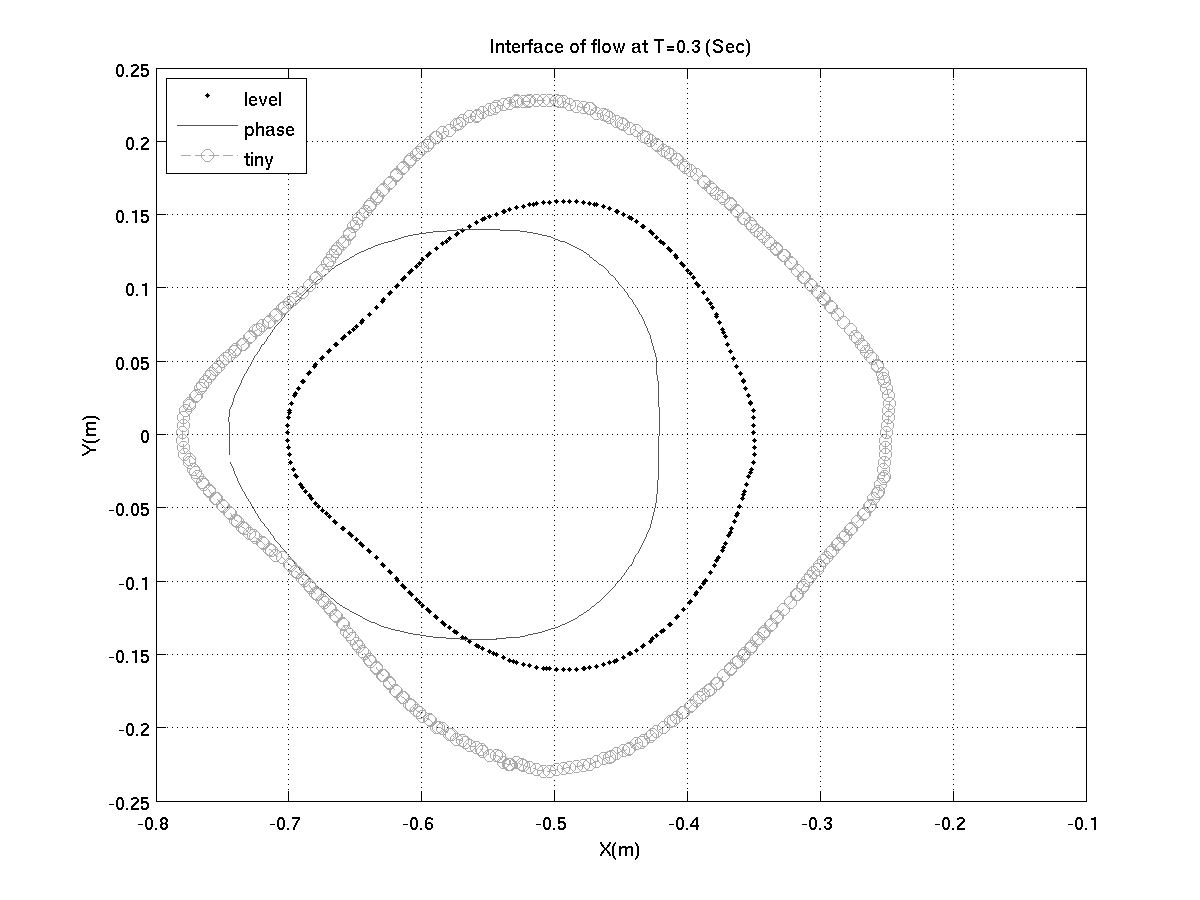
\includegraphics[width=1\textwidth]{IMAGES/interface30.png}
    \subcaption{T=0.3 sec}
  \end{minipage}
%   \hfill
  \begin{minipage}[b]{.48 \linewidth}
    \centering
    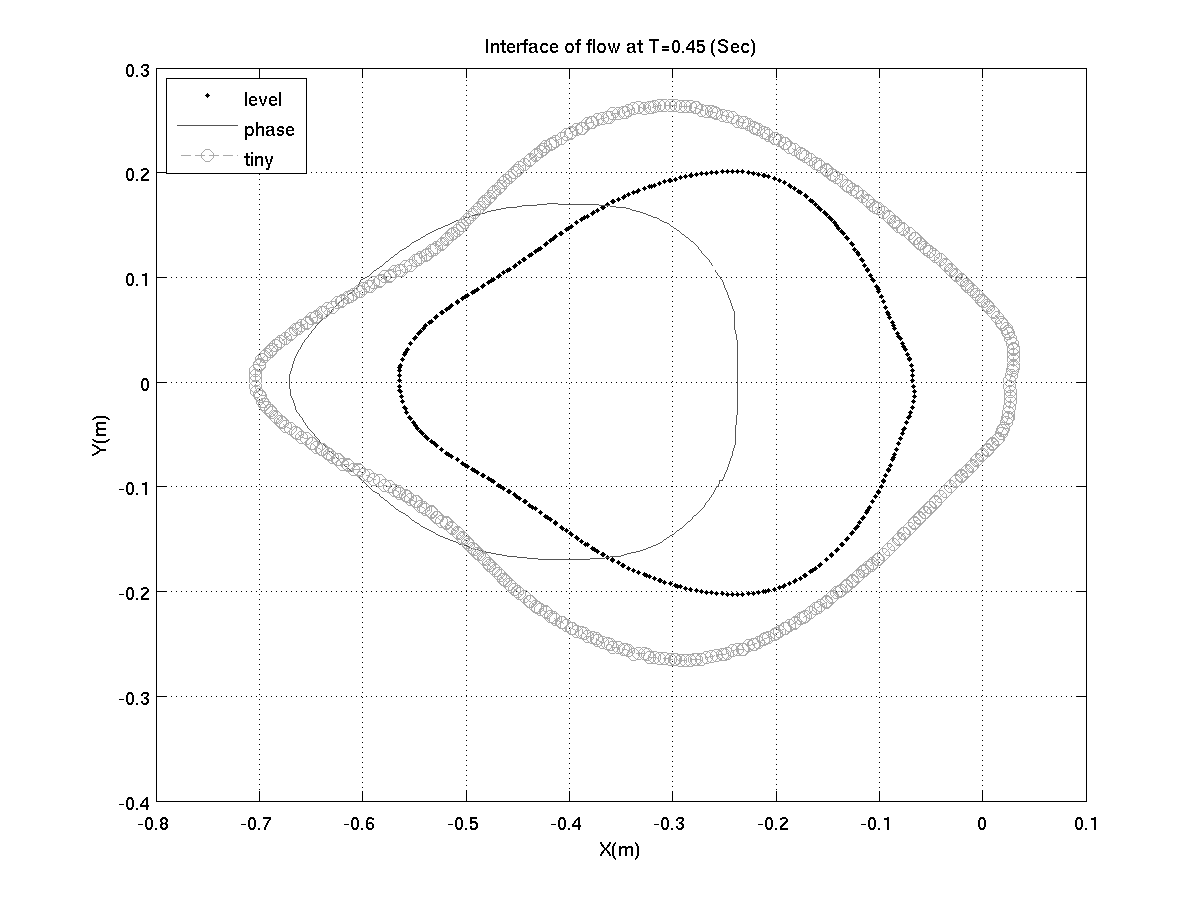
\includegraphics[width=1\textwidth]{IMAGES/interface45.png}
    \subcaption{T=0.45 sec}
    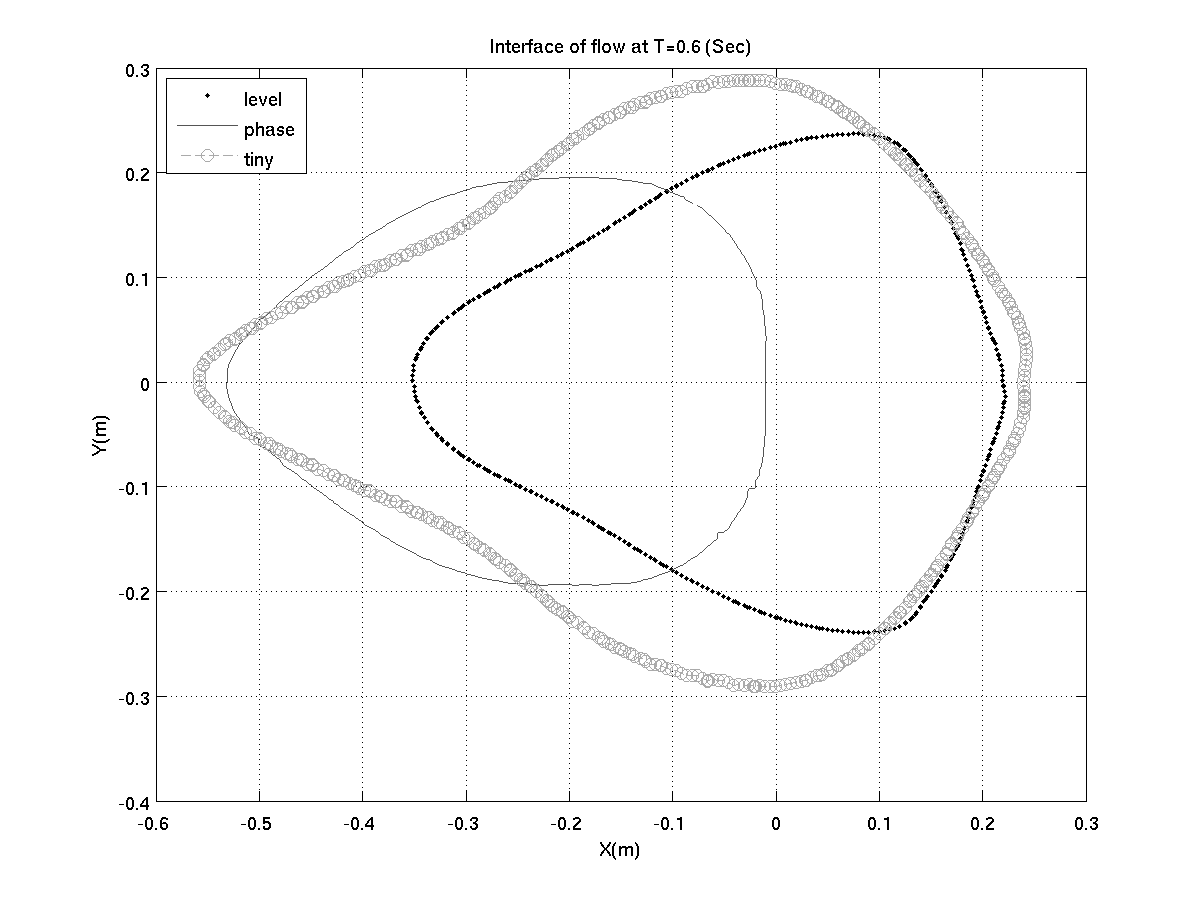
\includegraphics[width=1\textwidth]{IMAGES/interface60.png}
    \subcaption{T=0.6 sec}
  \end{minipage}
  \caption{Pile height contour and interface location at different time steps}
  \label{odinary}
\end{figure}

\subsubsection{Comparison}

For quantitative comparison of the results, we compared different schemes on three measurable quantities. The first measure is the extent of pile in X direction, the second one the extent of pile in Y direction, and the last one is the area of pile.

\begin{figure}[H]
  \begin{minipage}[b]{.48\linewidth}
    \centering
    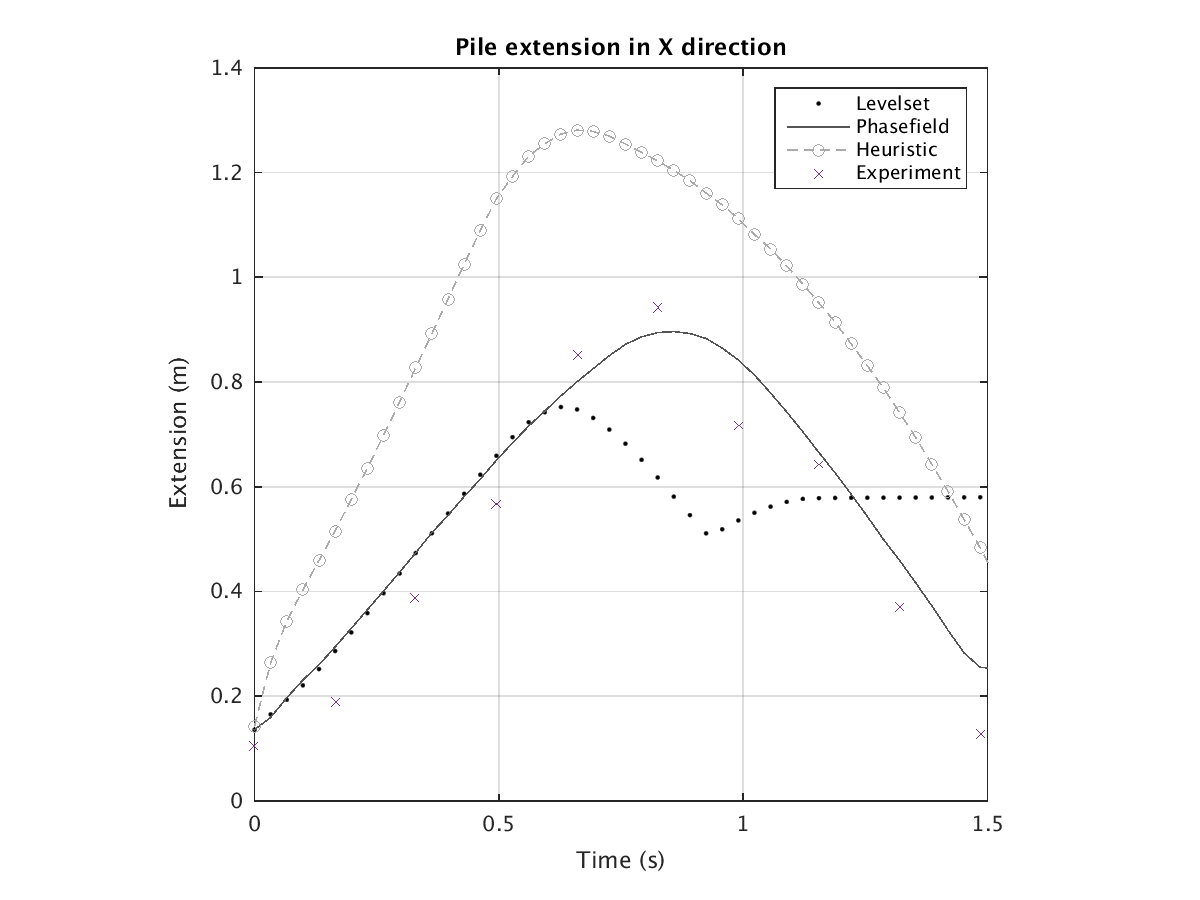
\includegraphics[scale=0.4]{IMAGES/xextend.png}
    \subcaption{Extension of pile in X direction}
    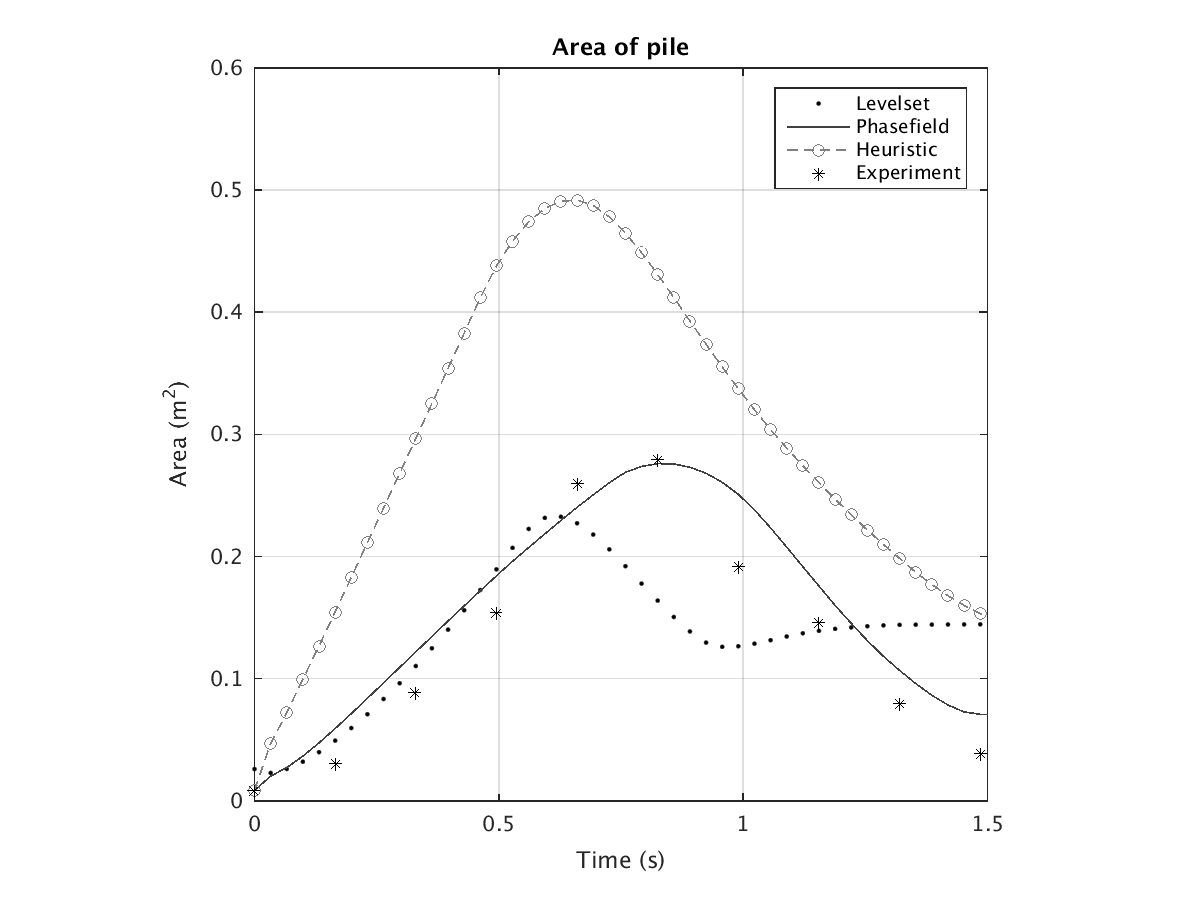
\includegraphics[scale=0.4]{IMAGES/area.png}
    \subcaption{Area of pile}
  \end{minipage}
%   \hfill
  \begin{minipage}[b]{.48 \linewidth}
    \centering
    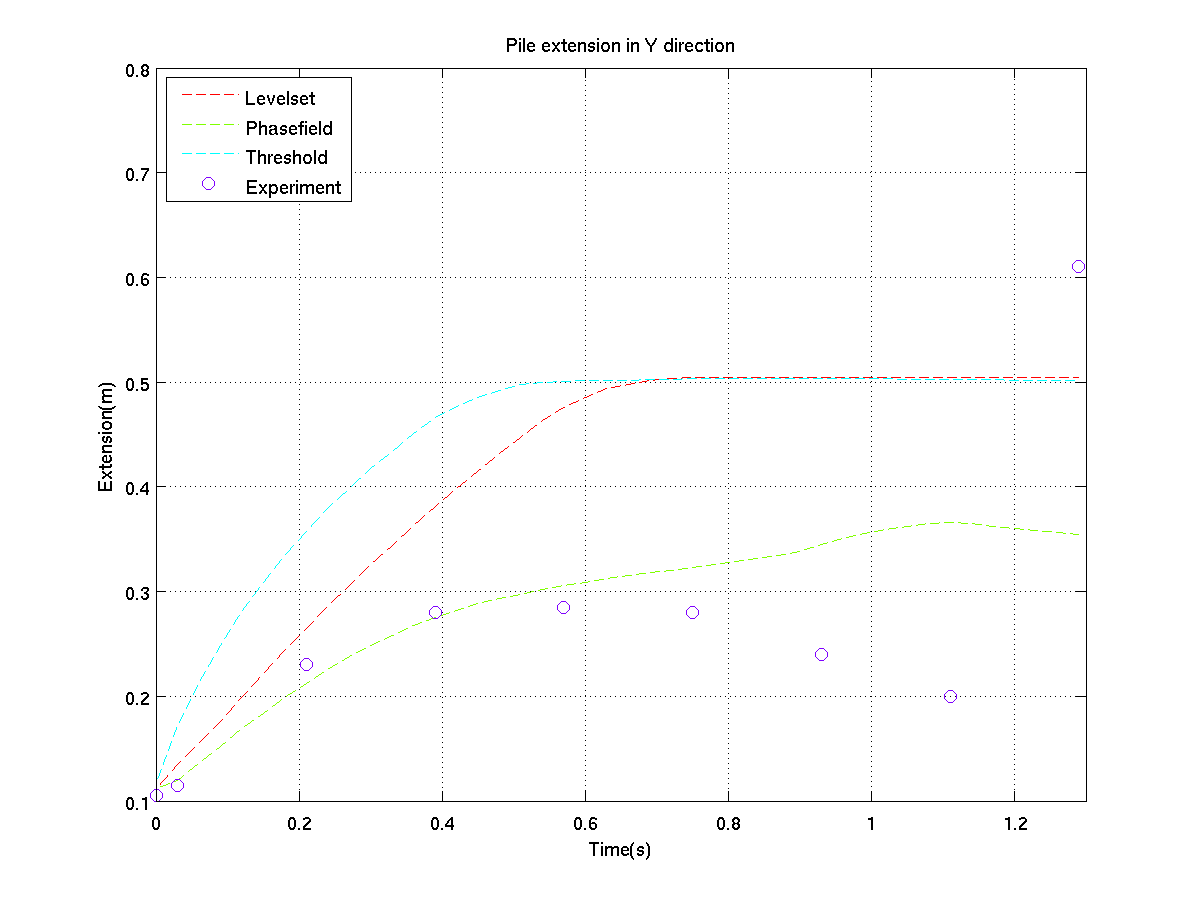
\includegraphics[scale=0.4]{IMAGES/yextend.png}
    \subcaption{Extension of pile in Y direction}
    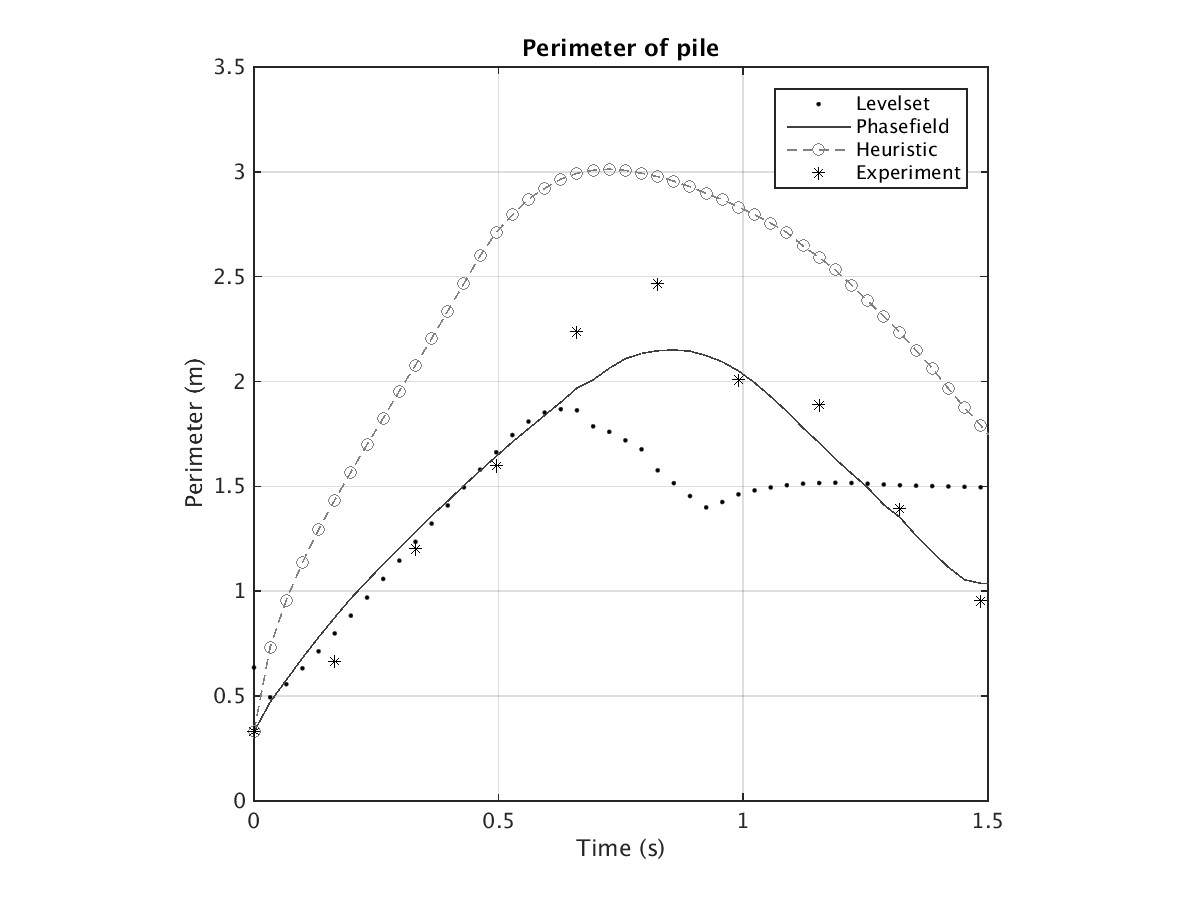
\includegraphics[scale=0.4]{IMAGES/perimeter.png}
    \subcaption{Perimeter of pile}
  \end{minipage}
  \caption{Comparison of the methods for flow on inclined plane}
  \label{compinc}
\end{figure}

% \end{figure}
\subsection{Colima Volcano}
In this section, we verify our different interface capturing methods with a field data of an eruption of Colima volcano. 
Colima volcano in Mexico is one of the most active volcano in North America, and this eruption has happened in 16-17 April 1991 \cite{Charbonnier2008}. 
The topography of Colima volcano is such that small changes the initial location of the pile leads to a completely different 
path of flow, so a good performance of any of the interface capturing methods for this case promises a reliable method for other volcanoes.
To be able to compare our results with the outline of deposit of flow, we record the history of all points with the finest 
resolution of the mesh during the simulation to check the points that are placed exactly on the boundary of the flow. 
As a definition boundary here means that the points that the flow passed from them, but has not passed one of their neighbors 
in different directions. For phase field and level set just with recording the maximum absolute value of $ \phi $ we can find 
these points by plotting $\phi=0$, this contour produces deposit line of flow during the time. For the heuristic method we 
recorded the minimum of the pile height during time and plotted the contour of $ h = h_{scale} \times GEOFLOW \_ TINY$, where 
$ h_{scale} =Volume^\frac{1}{3} $.

% \text{Height_Scale}
% \text{Height_Scale}
The resolution of the digital elevation model (DEM) of Colima volcano that here we used is 5 meter which is the finest DEM 
that we have ever used for this volcano.

The outline of this eruption is available in \cite{NamikawaPhD}, we used the method that described in \cite{NamikawaPhD} to 
extract the skeleton line of the flow to be able to compare the results quantitatively. The procedure of the extraction of the 
skeleton line is shown in the following pictures. 

\begin{figure}
        \centering
        \begin{subfigure}[b]{0.45\textwidth}
                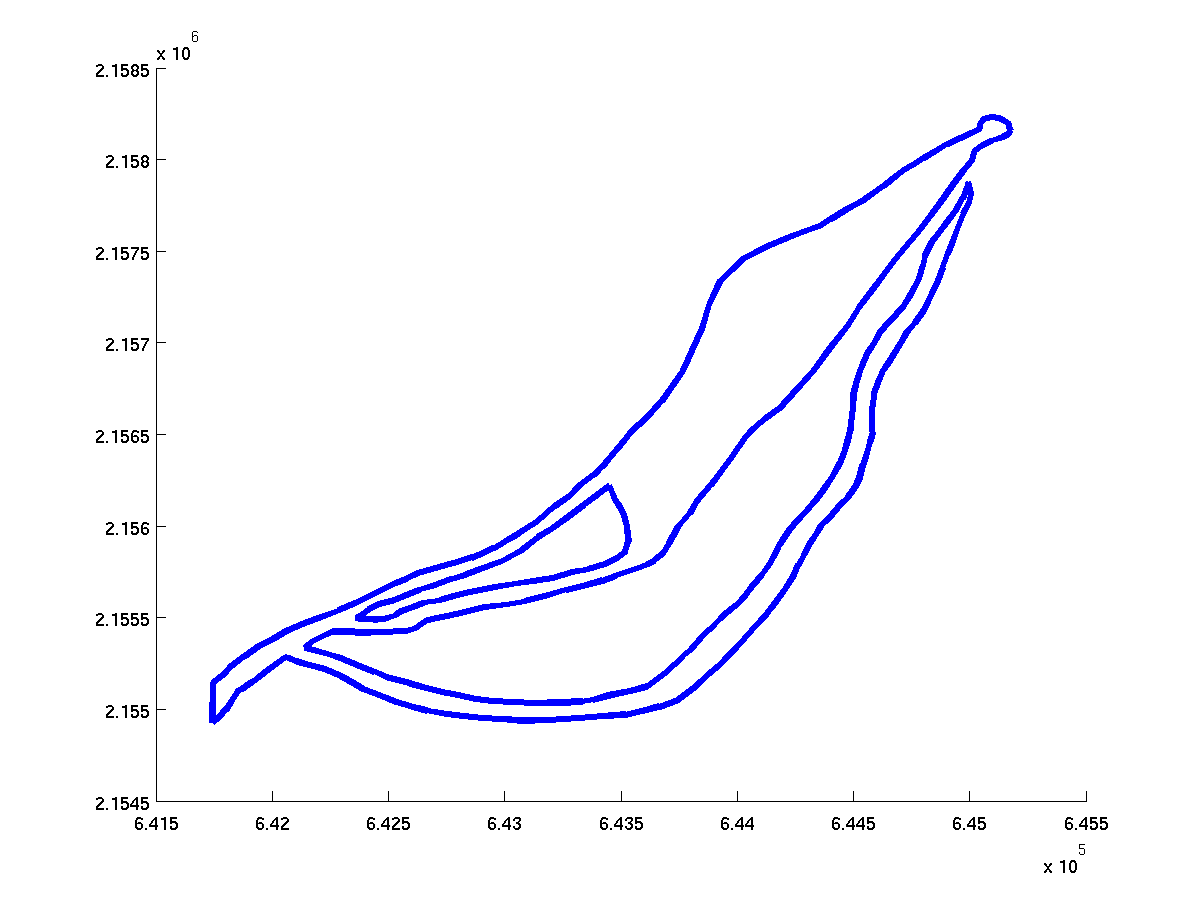
\includegraphics[width=\textwidth]{IMAGES/pics/outline.png}
                \caption{Outline of flow from field data}
                \label{fig:Outline}
        \end{subfigure}%
        \begin{subfigure}[b]{0.45\textwidth}
                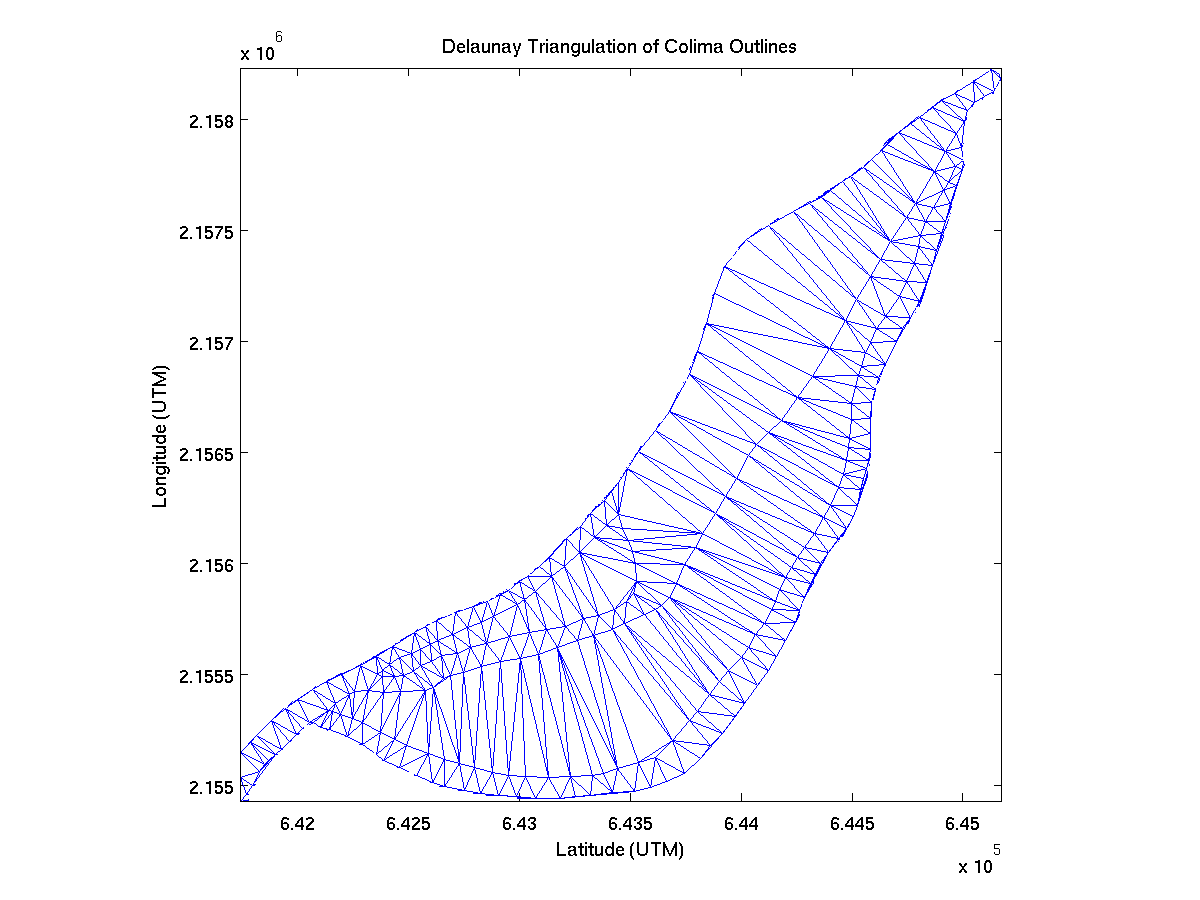
\includegraphics[width=\textwidth]{IMAGES/pics/Delaunay_Triangulation_of_Colima_clean.png}
                \caption{Delaunay triangulation based on the outline of the flow}
                \label{fig:Delaunay}
        \end{subfigure}\\
        \begin{subfigure}[b]{0.45\textwidth}
                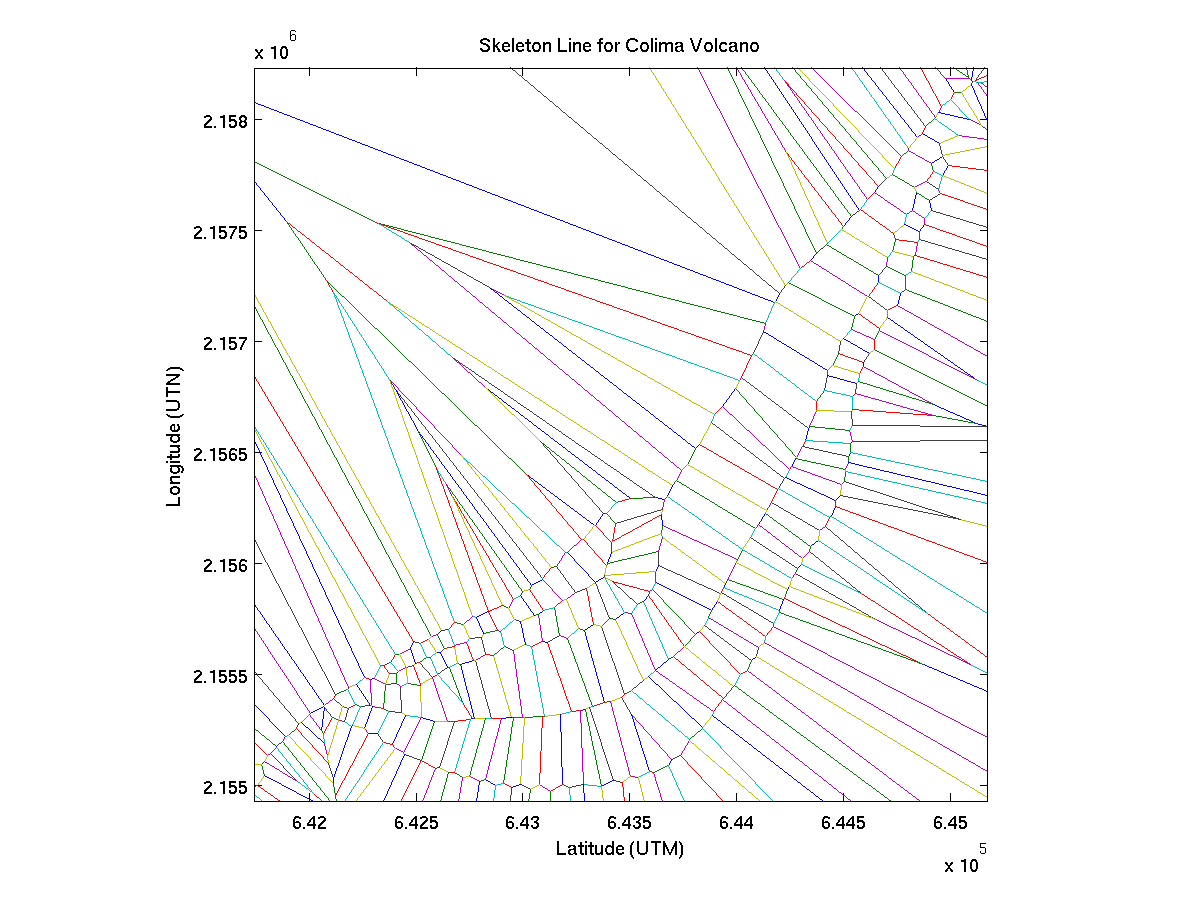
\includegraphics[width=\textwidth]{IMAGES/pics/Skeleton_line.png}
                \caption{Finding the middle of the edges of the triangles that connects the outline of the flow}
                \label{fig:veroni}
        \end{subfigure}
        \begin{subfigure}[b]{0.45\textwidth}
                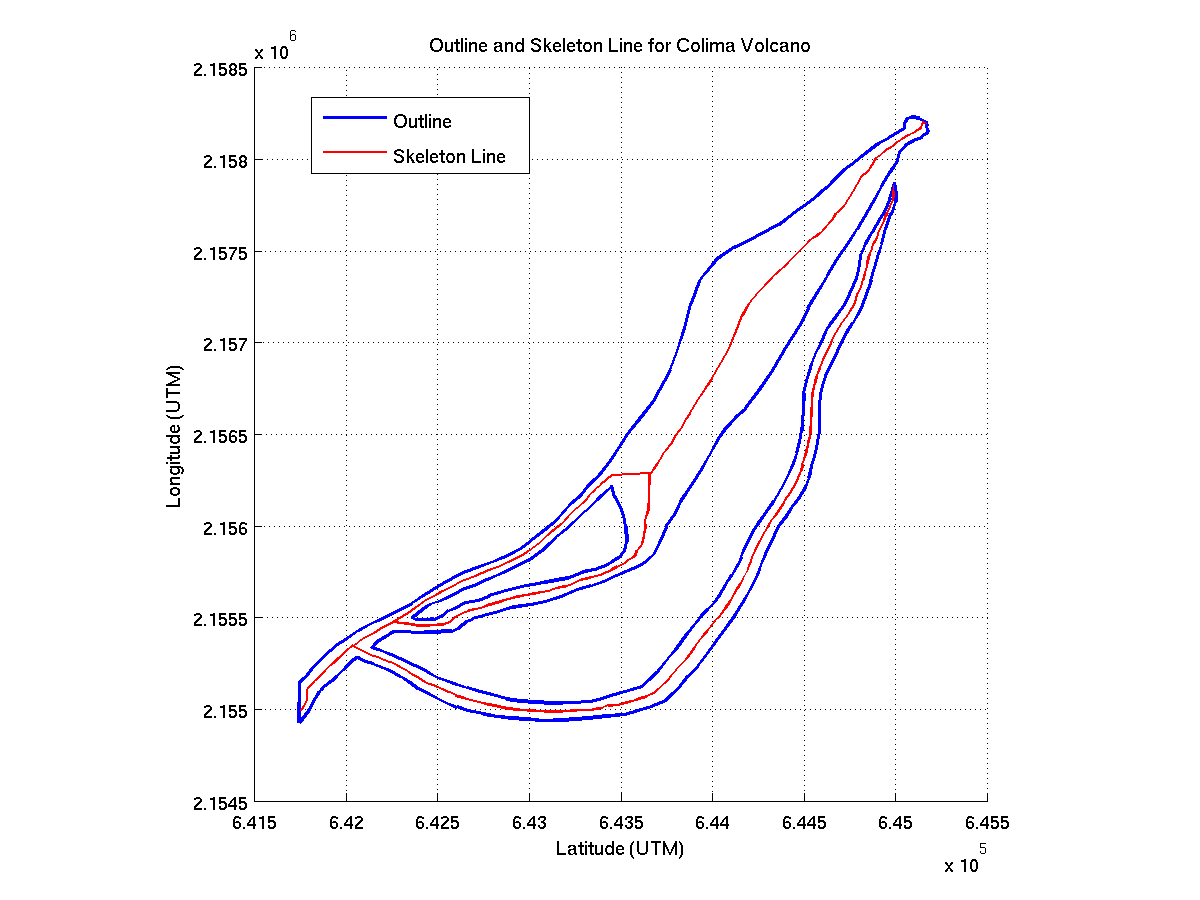
\includegraphics[width=\textwidth]{IMAGES/pics/Outline_Skeleton_line.png}
                \caption{Connecting the middle verticals that are inside of the outline of the flow, in this picture the
                outline of the flow (blue line) and the skeleton line of the flow (red line) can be seen}
                \label{fig:skeleton}
        \end{subfigure}
                
        \caption{In this set of pictures the steps that have to be taken for finding the outline of the flow is displayed 
        respectively}\label{fig:skeleton_line_proc}
\end{figure}

%\newpage

After finding the skeleton line, we mapped the outline of the flow and the skeleton line on the Colima volcano 
using KML language and Google earth application \ref{skel_outline}. In figure \ref{Colimapic} the result of each methods and their comparison can be seen. 

\begin{figure}[H]
\centerline{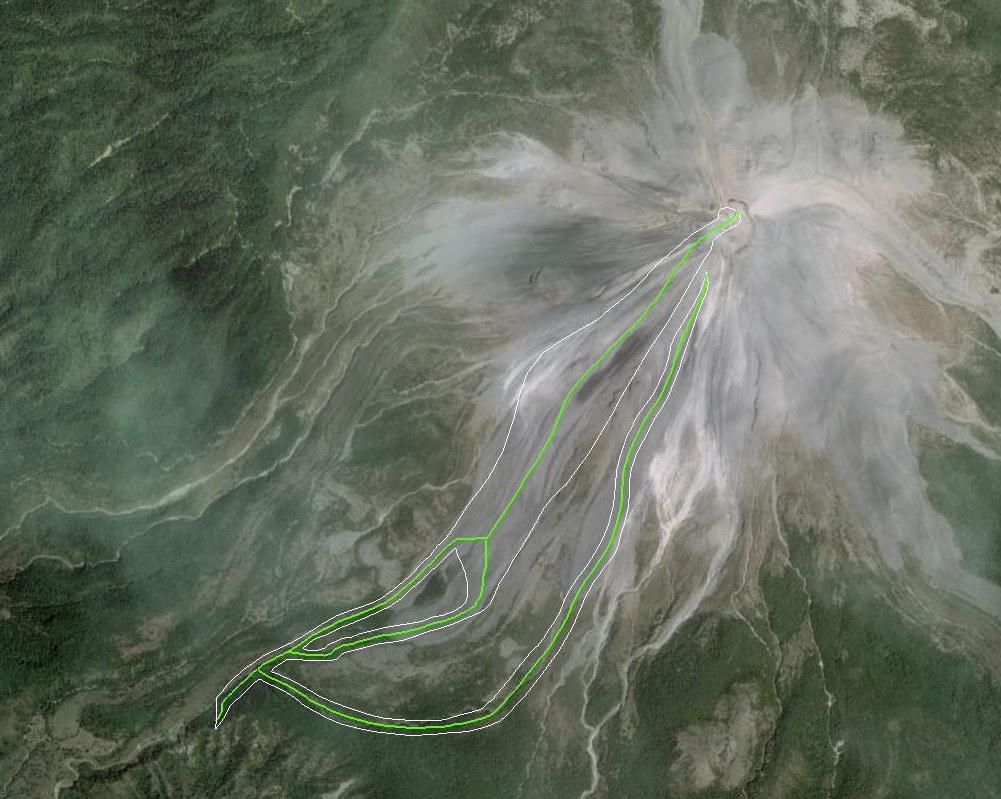
\includegraphics[width=.35\textwidth]{IMAGES/skeleton_outline1.jpg}}
\caption{Skeleton line (white line) and outline of the deposit of eruption 1991 (yellow line)}
\label{skel_outline}
\end{figure}

\begin{figure}[H]
  \begin{minipage}[b]{.48\linewidth}
    \centering
    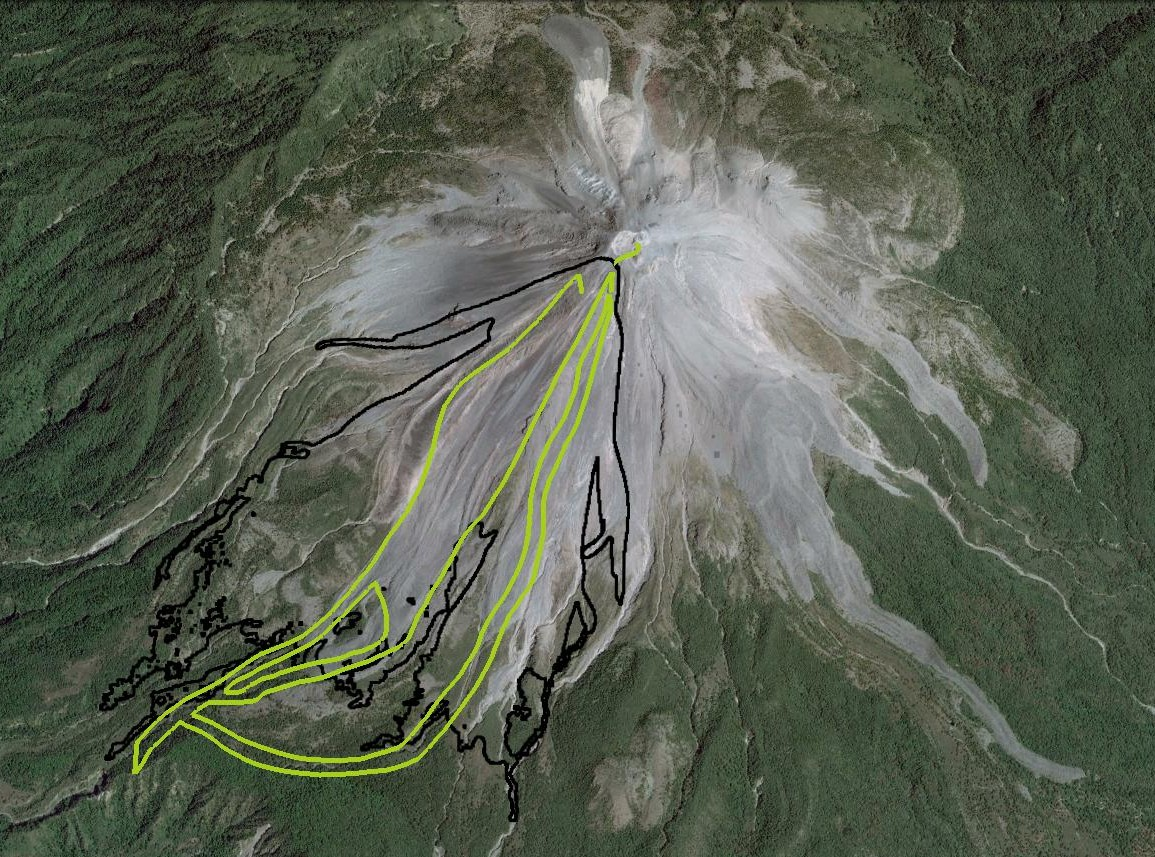
\includegraphics[width=.95\textwidth]{IMAGES/tiny1.jpg}
    \subcaption{Outline from Heuristic Method}
    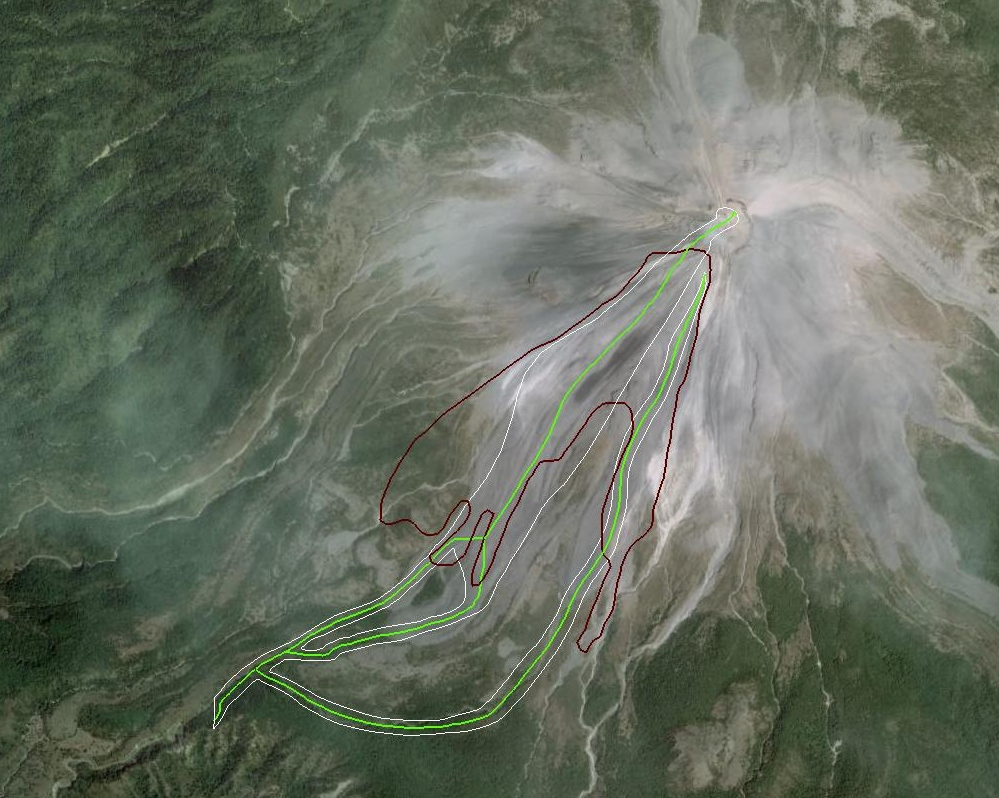
\includegraphics[width=.95\textwidth]{IMAGES/levelset1.jpg}
    \subcaption{Outline from Level set Method}
  \end{minipage}
%   \hfill
  \begin{minipage}[b]{.48 \linewidth}
    \centering
    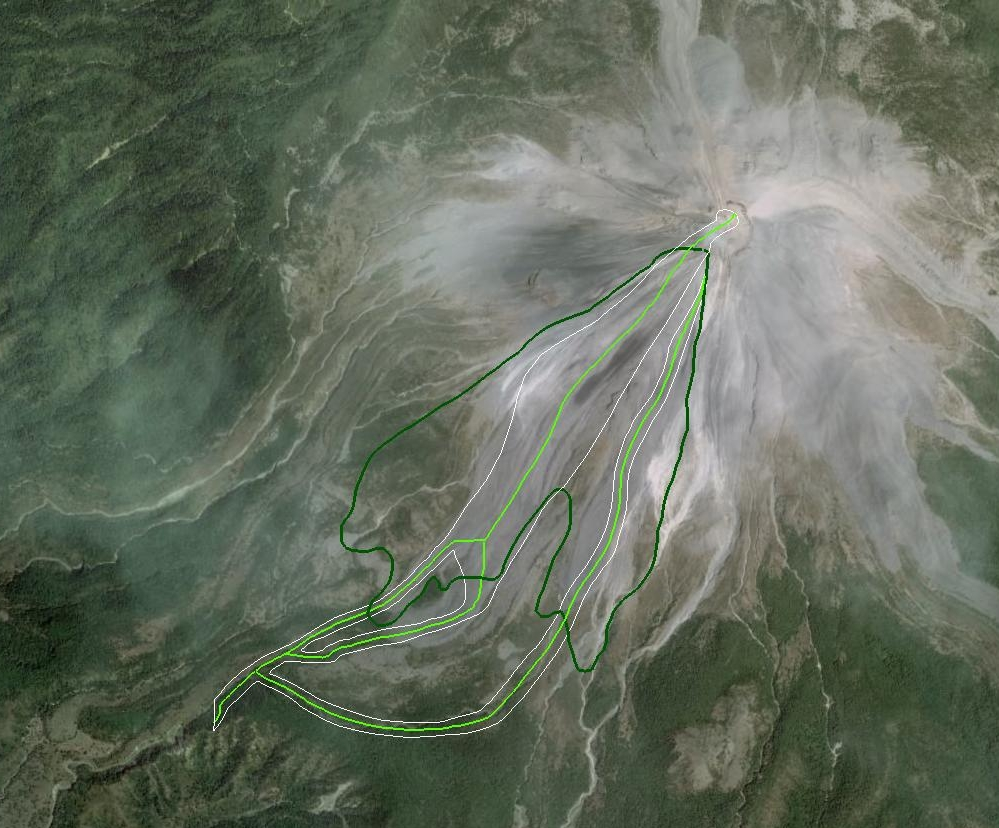
\includegraphics[width=.95\textwidth]{IMAGES/phasefield1.jpg}
    \subcaption{Outline from Phase field Method}
    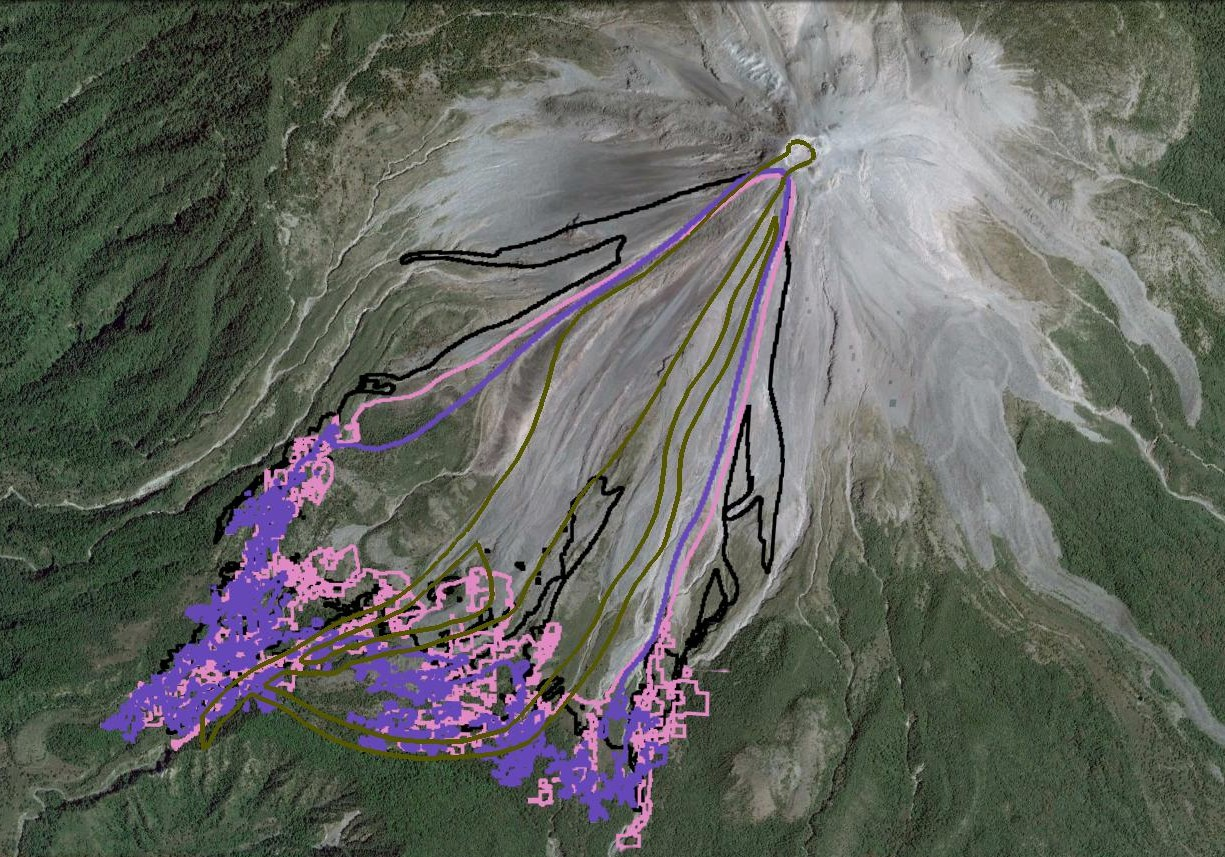
\includegraphics[width=.95\textwidth]{IMAGES/comparison1.jpg}
    \subcaption{Comparison of all three methods}
  \end{minipage}
  \caption{Comparison of the obtained outline of flow from Heuristic, Level set, and Phase field methods for Colima Volcano}
  \label{Colimapic}
\end{figure}

%\begin{figure}[H]
%\centerline{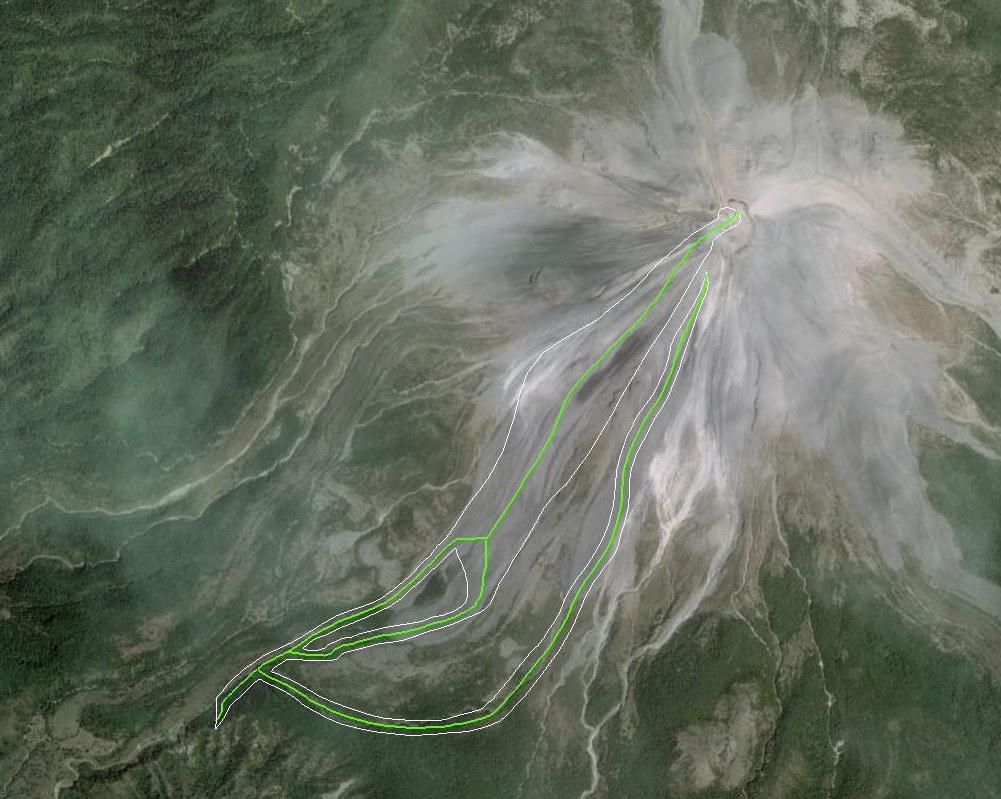
\includegraphics[width=.5\textwidth]{IMAGES/skeleton_outline1.jpg}}
%\caption{Skeleton line (white line) and outline of the deposit of eruption 1991 (yellow line)}
%\label{skel_outline}
%\end{figure}
%
%\begin{figure}[H]
%\centerline{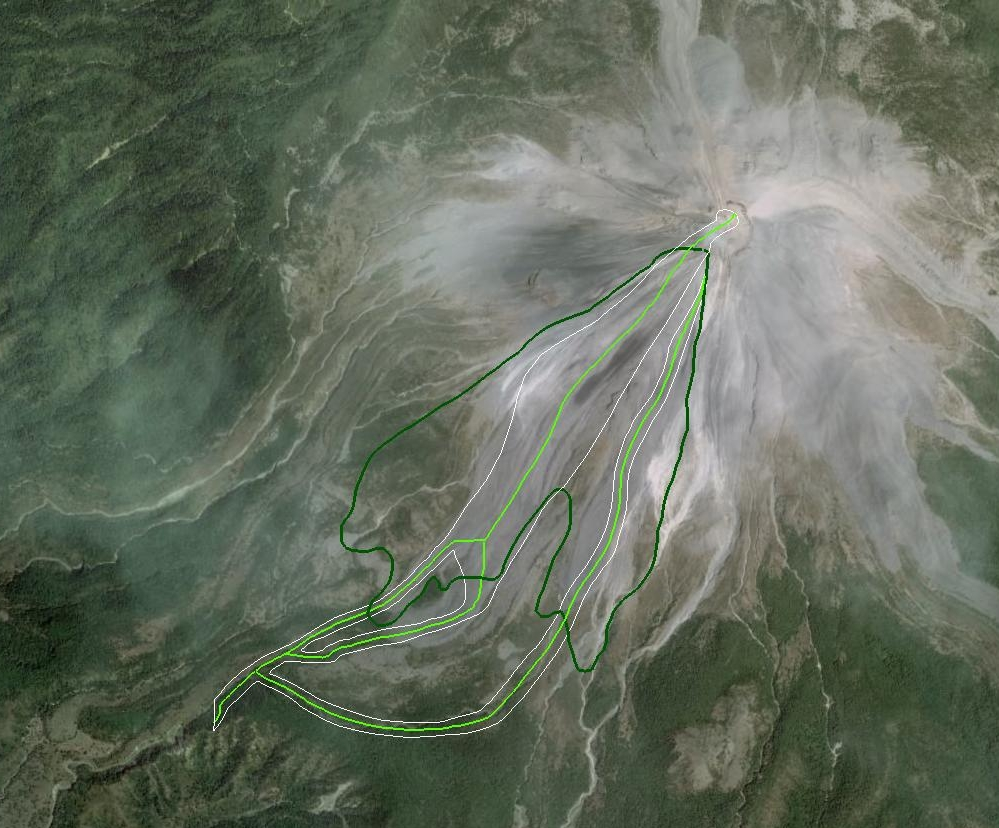
\includegraphics[width=.5\textwidth]{IMAGES/phasefield1.jpg}}
%\caption{}
%\label{phasecolima}
%\end{figure}
%
%\begin{figure}[H]
%\centerline{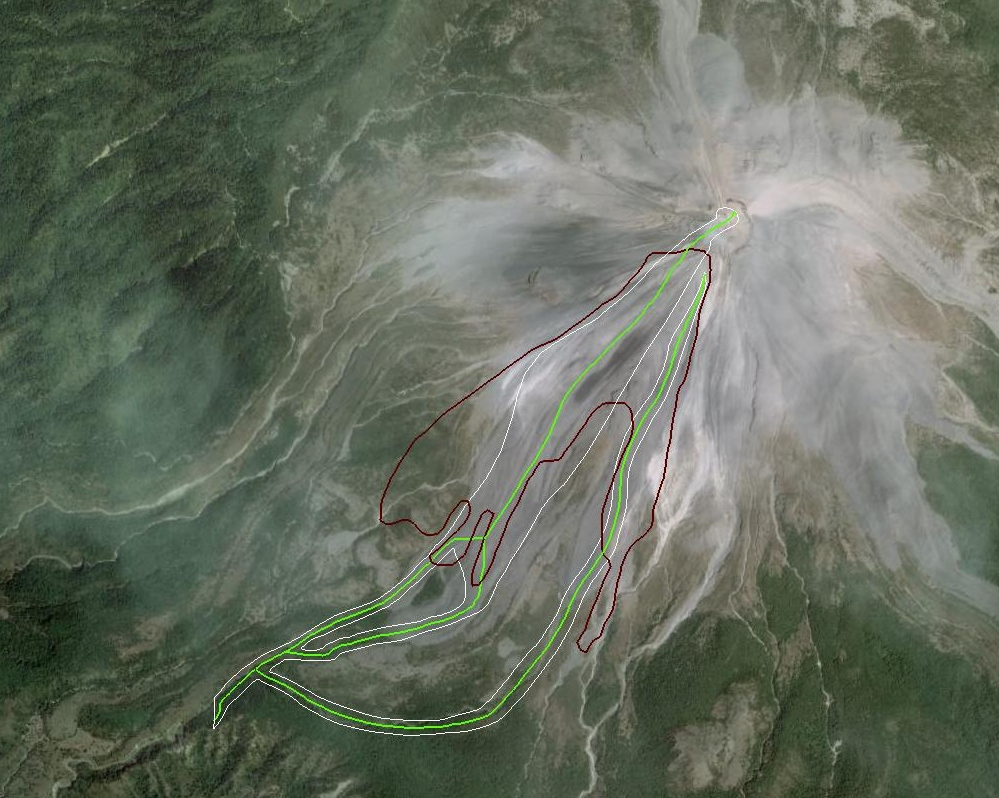
\includegraphics[width=.5\textwidth]{IMAGES/levelset1.jpg}}
%\caption{Skeleton line (white line) and outline of the deposit of eruption 1991 (yellow line)}
%\label{level_colima}
%\end{figure}
% 
% \begin{figure}[H]
% \centerline{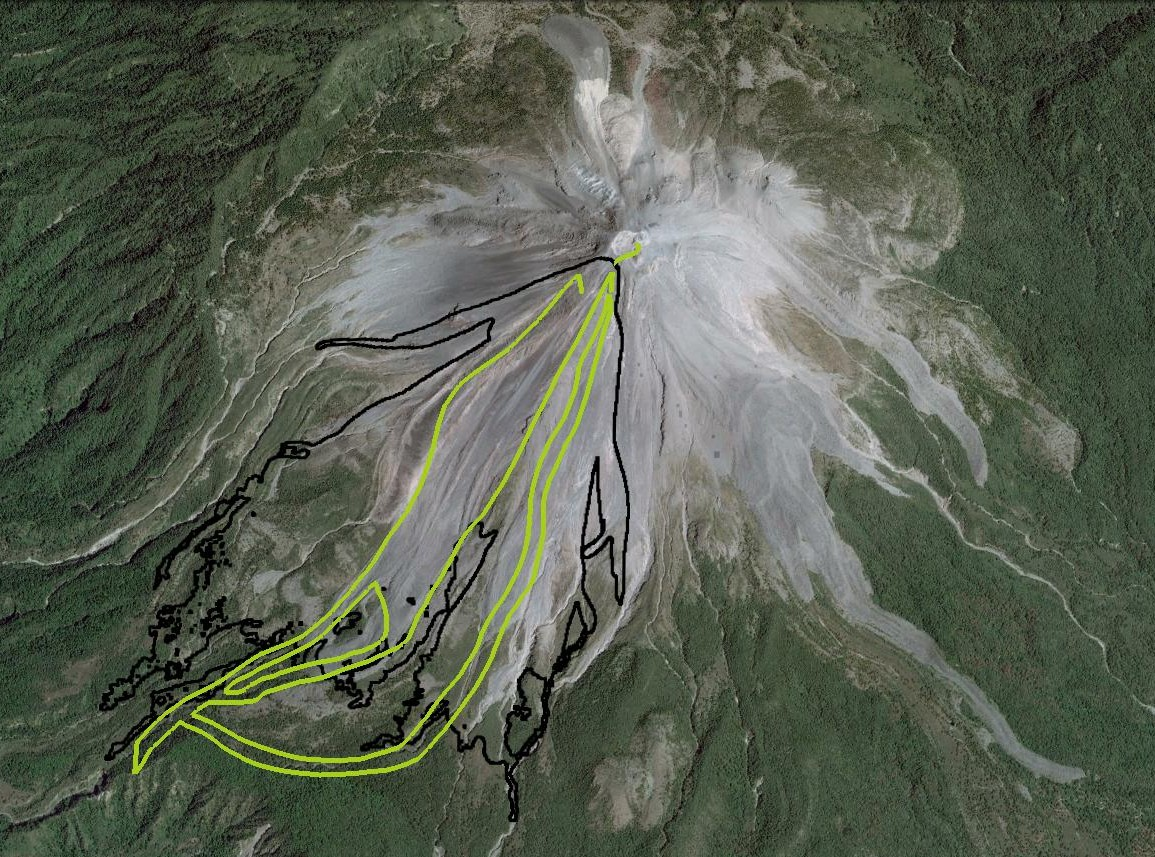
\includegraphics[width=.5\textwidth]{IMAGES/tiny1.jpg}}
% \caption{Skeleton line (white line) and outline of the deposit of erution 1991 (yellow line)}
% \label{tiny_colima}
% \end{figure}
% 
% \begin{figure}[H]
% \centerline{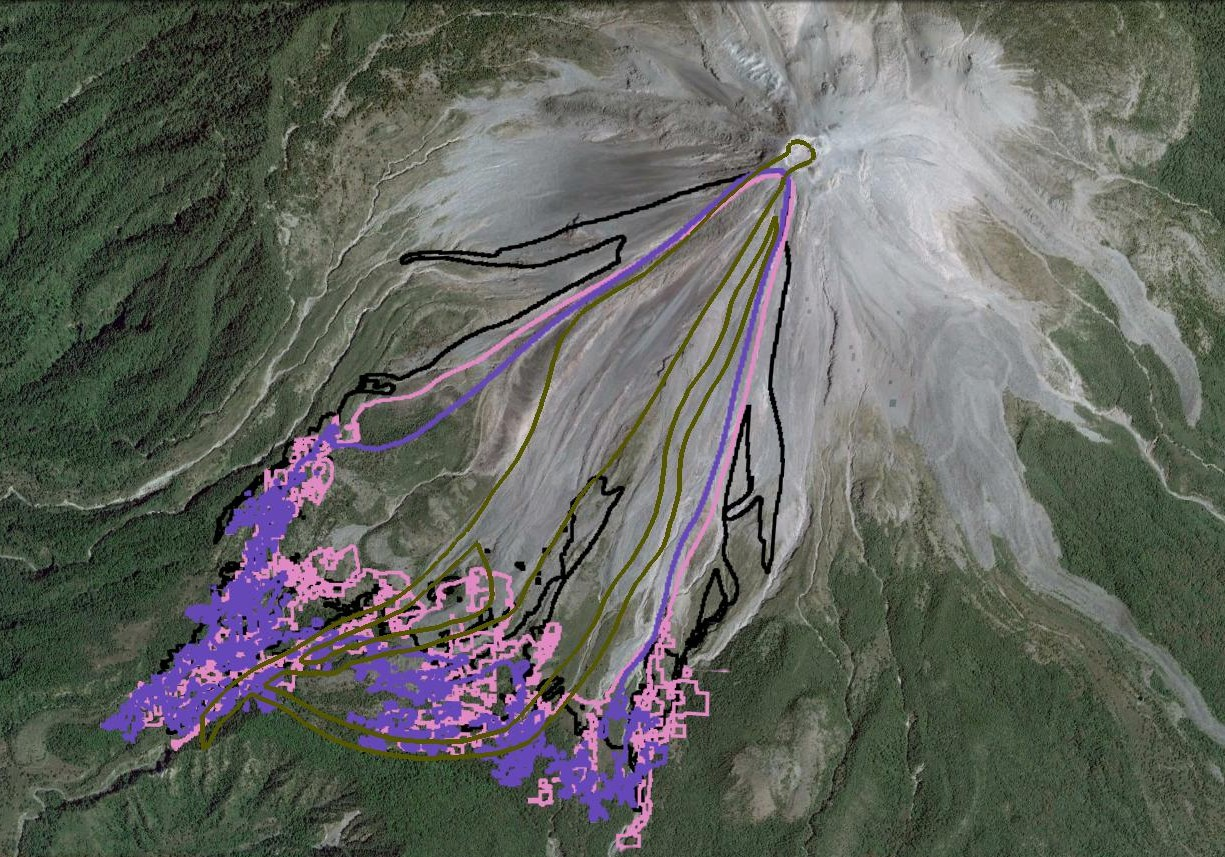
\includegraphics[width=.5\textwidth]{IMAGES/comparison1.jpg}}
% \caption{Skeleton line (white line) and outline of the deposit of erution 1991 (yellow line)}
% \label{compfig}
% \end{figure}



\section{Conclusions} \label{conclusions}
The numerical solution of the Savage-Hutter (and similar 
``shallow-water'') equations have historically been plagued by 
several interrelated numerical difficulties which are collectively 
characterized by a non-physically thin-layer extending 
large distances from the realistic main body of the flow. In the 
best case, this ``thin-layer problem'' means a ``no flow'' boundary 
line must be arbitrarily drawn at some given depth contour.  In 
the worst case, it can cause severe numerical instability that 
prevents any simulation of a particular event.

In this paper, we 
have described some features of the thin-layer problem,
some underlying causes that are common to virtually all numerical 
solution methodologies.  Moreover, we have presented a heuristic method and compared 
two interface capturing approaches that 
mitigate this problem by addressing its root causes.  We 
implemented these thin-layer control strategies in TITAN2D, our high 
performance finite volume solver of the depth-averaged granular 
flow equations.  Numerical simulations were performed for 
geophysical mass flows at two separate locations.

The numerical experiment were conducted for an inclined plate that finally continues horizantally. 
This case was tested with all of the approaches,
which not only prevented the 
loss of numerical stability but also demonstrated behavior that
is, at least qualitatively, consistent with expectations.

The second location, Colima volcano, which is an active volcano 
in Mexico, was selected on the basis that the DEM had provoked 
thin-layer numerical difficulties from an earlier version of TITAN2D, 
and that a campanologist familiar with the location had selectively 
tuned TITAN2D's few input parameters and also computational and 
post-processing thresholds to produce results that closely matched 
reality for that location. The new version of TITAN2D, which implemented
our thin-layer control strategy, automatically (i.e. without 
tuning) reproduced a flow outline that had even greater agreement 
with the historical data. 

Then the results of these approaches were compared. The result of this comparison showed 
a very good consistency between these approaches.
% Therefore the phase field method could be used for finding the flow boundary 
% of flow and handle the WD problem. 

On the basis of these very positive results, we concluded that our 
thin-layer control strategy, and interface capturing approach provides sufficient benefit. 
While all of these approaches to thin-layer mitigation was developed in the 
context of TITAN2D's capabilities, much of it should be appropriate 
for use in depth-averaged flow solvers with different numerical 
implementations.

\newpage
\appendix
\section{Appendix 1} \label{app1}

The constrain that we want to satisfy is to preserve the mass for entire flow. Since this flow is an incompressible flow, we can write:
\begin{equation} 
\frac{D}{Dt} \int_\Omega \varphi h \ \ dx= 0.
\end{equation}

with using Reynold's theorem, we can expand the above integral in to:

\begin{equation} \label{reycons}
\int_\Omega \frac{\partial (\varphi h)}{\partial t} \ dx + \int_\Gamma (\overrightarrow{V}.\overrightarrow{n}) (\varphi h)\  ds = 0,
\end{equation}

where $ \Gamma $ is the boundary of $\Omega$, and $\overrightarrow{n}$ is its normal vector, and $\overrightarrow{V}$ is velocity vector. The boundary and initial conditions for $\varphi$ and velocity are:

\begin{gather*} 
\overrightarrow{V}_{t=0}=\overrightarrow{V}_0(\textbf{x}), \ \ \ 
\varphi_{t=0}=\varphi_0(\textbf{x}), \ \ \ \ x\in \Omega \\
\frac{\partial \varphi}{\partial n}\vert_{\Gamma} = 0.
\end{gather*}
With the above initial and boundary conditions, and Gauss' identity, the equation \eqref{reycons} can be written:
\begin{equation}
\label{expand}
\underbrace{\int_\Omega \varphi \frac{\partial h}{\partial t} dx}_\text{a} + 
\underbrace{\int_\Omega h \frac{\partial \varphi}{\partial t} dx}_\text{b} +
\underbrace{\int_\Omega \varphi \nabla.(h\overrightarrow{V}) dx}_\text{c} +
\underbrace{\int_\Omega h\overrightarrow{V}.\nabla \varphi }_\text{d}
= 0.
\end{equation}

We know $a+c=0$ from conservation of mass (equation \eqref{governingeq}), so   $b+d=0$:
\begin{equation}
\label{expand1}
 \int_\Omega h (\frac{\partial \varphi}{\partial t} \  + \
\overrightarrow{V}.\nabla \varphi) \ \ dx = 0.
\end{equation}

Since in the above equation, the expression inside the preanthesis is the LHS of phase field equation \eqref{allencahn}, we can substitute it with the RHS of the same equation, so:

\begin{equation}
\label{rhssubs}
 \int_\Omega h (\frac{\partial \varphi}{\partial t} \  + \
\overrightarrow{V}.\nabla \varphi) \ \ dx = 
\int_\Omega h \gamma (\bigtriangleup \varphi -F'(\varphi)+\xi(t))  \ \ dx \ = 0 .
\end{equation}

Applying the Gauss' theorem on laplacian term, with considering the boundary conditions on $\varphi$:

\begin{equation}
\label{lapbound}
 \int_\Omega h \gamma  \nabla. \nabla \varphi \ dx = 
 \int_\Gamma h \gamma \nabla \varphi \ ds = 0,
\end{equation}
consequently equation \eqref{rhssubs} leads to:
\begin{equation}
\label{xitcon}
\xi(t)  \int_\Omega h  \ dx = 
 \int_\Gamma h F'(\varphi) dx, 
 \end{equation}


and we know intial volume is equal to $\int_\Omega h  \ dx $, therefore we can conclude:
\begin{equation}
\label{finalxi}
\xi(t)  = \frac{1}{V_0} \int_\Gamma h F'(\varphi) dx. 
 \end{equation}

 
\bibliographystyle{plain}
\bibliography{mybib}
\end{document}
